\chapter{Modelado}

En este capítulo presento solamente el modelo final desarrollado en la tesis conjunta {\color{Red} Tesis Actuaría}, el lector interesado en la discusión de dicho modelo puede referirse a la versión completa. Ahora bien, mi objetivo era explorar las configuraciones sociales que favorecieron o inhibieron el voto por el FN en 2012. Por ello, hay que notar que los datos electorales que considero son el número de votos por Marine Le Pen en cada comuna así como el número de inscritos en el listado nominal de las mismas. Tenemos entonces $C$ pares de la forma $\left\lbrace y_c, n_c \right\rbrace$ donde $y_c$ representa el número de votos y $n_c$ el de inscritos en la comuna $c \,\in\,\mathbb{N}_C$. Este tipo de datos puede ser modelado como proveniente de una distribución binomial con número de ensayos conocido y parámetro de interés $p_c$: 
\begin{equation*}
y_c|p_c \sim Binom(n_c, p_c) \quad \forall \; c \, \in \mathbb{N}_C
\end{equation*} 

Podemos interpretar cada parámetro $p_c$ como la afinidad que se tuvo en la comuna $c$ por Marine Le Pen en la primera vuelta presidencial de 2012. Esta afinidad es la que quisiéramos explicar en términos de configuraciones sociales.\\

Una regresión binomial con liga logística, comunmente conocida como regresión logística, con un vector $x_c$ de variables explicativas en la comuna $c$, puede construirse de la siguiente manera: 
\begin{align*}
y_c|\theta & \sim Binom(n_c,p_c) \quad \forall \quad c \in \mathbb{N}_C \\
\text{con} \quad \log\left(\dfrac{p_c}{1-p_c}\right) &= \alpha + \beta x_c \nonumber \\
\text{y} \quad \theta &= (\alpha,\beta) \sim f(\theta),
\end{align*}
donde $f(\theta)$ representa nuestro conocimiento inicial en un modelo bayesiano.\\ 

En nuestro caso tenemos $m$ variables censales formadas, cada una, por distintas categorías poblacionales. Sin pérdida de generalidad, para la $m$-ésima variable censal tenemos un vector de proporciones $x_{m,c}=(x_{m,1,c},\dots,x_{m,l_m,c})$ donde $l_m$ es el número de categorías de la variable y $\sum\limits_{j=1}^{l_m} x_{m,j,c}=1$. Debido al problema de multicolinealidad que esto ocasionaría, defino una restricción de identificabilidad de suma cero para los coeficientes, de manera tal que $\sum\limits_{j=1}^{l_m}\beta_j=0$.\\

Por otro lado, el análisis exploratorio de datos sugería que se podría modelar de mejor manera dejando que los coeficientes e interceptos variasen para cada uno de los 96 departamentos. Si denotamos como $d[c]$ el \textit{departamento} al que pertenece la comuna $c$, un ejemplo de modelo jerárquico para nuestro caso sería: 
\begin{align}\label{eq:Modelo_Jer_Ind}
y_c|\theta & \sim Binom(n_c,p_c) \quad \forall \, c \in \mathbb{N}_C \nonumber \\
\text{con} \quad \log\left(\dfrac{p_c}{1-p_c}\right) &= \alpha_{d[c]} + \sum\limits_{j=1}^{l_m} \beta_{d[c],j} x_{m,j,c} \nonumber\\ 
\text{tal que} \quad -\sum\limits_{j = 1}^{l_m} \beta_{d,j} &= 0 \nonumber \\
\alpha_d & \sim N(\mu_{\alpha}, 1) \quad \forall \, d \in \mathbb{N}_{96} \nonumber \\
\beta_{d,j} & \sim N(\mu_{\beta}, 1) \quad \forall \, j \in \mathbb{N}_{l_m-1}  \quad \text{y} \quad d \in \mathbb{N}_{96} \nonumber \\
\mu_{\alpha} &\sim N(-1.7, 0.25^2) \nonumber \\
\mu_{\beta} &\sim N(0,0.5^2)
\end{align}

Sin embargo, cuento con distintas variables y no solo una $x_m$. Así pues, podemos hablar de la composición de la comuna por escolaridad como una variable $x_{escol,c}$ y de la misma manera para las categorías socioprofesionales, los grupos de edad, la condición migratoria, el sexo y las ocupaciones por edades. Al final, el modelo final de la tesis completa es el siguiente: 

\begin{align}\label{eq:Modelo_Comp_H}
y_c|\theta & \sim Binom(n_c,p_c) \quad \forall \, c \in \mathbb{N}_C \nonumber \\
\begin{split}
\text{con} \quad ln\left(\dfrac{p_c}{1-p_c}\right) &= \alpha_{d[c]} + \beta_{d[c]} x_{escol,c} + \gamma_{d[c]} x_{csp,c} + \delta_{d[c]} x_{edad,c} + \lambda_{d[c]} x_{migr,c} \\
&+ \kappa_{d[c]} x_{sexo,c} + \zeta_{d[c]} x_{ocu\_gral,c} + \xi_{d[c]} x_{ocu\_juv,c} + \upsilon_{d[c]} x_{ocu\_may,c} 
\end{split}\\
\shortintertext{tal que} 
\beta_{d,5} &= -\sum\limits_{k = 1}^{4} \beta_{d,k}, \nonumber \\
\gamma_{d,8} &= -\sum\limits_{k = 1}^{7} \gamma_{d,k} \nonumber \\
\delta_{d,6} &= -\sum\limits_{k = 1}^{5} \delta_{d,k} \nonumber \\
\lambda_{d,2} &= -\lambda_{d,1} \nonumber \\
\kappa_{d,2} &= -\kappa_{d,1} \nonumber \\
\zeta_{d,2} &= -\zeta_{d,1} \nonumber \\
\xi_{d,2} &= -\xi_{d,1} \nonumber \\
\upsilon_{d,2} &= -\upsilon_{d,1} \nonumber \\
\shortintertext{donde $\forall \, d \in \mathbb{N}_{96}$}
\alpha_d &\sim N(\mu_{\alpha}, \sigma=1) \quad  \nonumber \\
\beta_{d,j} &\sim N(\mu_{\beta}, \sigma=1) \quad \forall \, j \in \mathbb{N}_{4} \nonumber \\
\gamma_{d,j} &\sim N(\mu_{\gamma}, \sigma=1) \quad \forall \, j \in \mathbb{N}_{7} \nonumber \\
\delta_{d,j} &\sim N(\mu_{\delta}, \sigma=1) \quad \forall \, j \in \mathbb{N}_{5}  \nonumber \\ 
\lambda_{d,1} &\sim N(\mu_{\lambda}, \sigma=1) \nonumber \\
\kappa_{d,1} &\sim N(\mu_{\kappa}, \sigma=1) \nonumber \\ 
\zeta_{d,1} &\sim N(\mu_{\zeta}, \sigma=1) \nonumber \\
\xi_{d,1} &\sim N(\mu_{\xi}, \sigma=1) \nonumber \\
\upsilon_{d,1} &\sim N(\mu_{\upsilon}, \sigma=1) \nonumber \\
\shortintertext{y}
\mu_{\alpha} &\sim N(-1.7,\sigma=0.25) \nonumber \\
\mu_{\beta} &\sim N(0,\sigma=0.5) \nonumber \\
\mu_{\gamma} &\sim N(0,\sigma=0.5) \nonumber \\
\mu_{\delta} &\sim N(0,\sigma=0.5) \nonumber \\
\mu_{\lambda} &\sim N(0,\sigma=0.5) \nonumber \\
\mu_{\kappa} &\sim N(0,\sigma=0.5) \nonumber \\
\mu_{\zeta} &\sim N(0,\sigma=0.5) \nonumber \\
\mu_{\xi} &\sim N(0,\sigma=0.5) \nonumber \\
\mu_{\upsilon} &\sim N(0,\sigma=0.5) \nonumber
\end{align}

Después de ajustarlo mediante el software Stan, obtuve las distribuciones posteriores dada la muestra de datos discutida en la \textbf{\autoref{secc:muestra}}. Una vez con dichas distribuciones posteriores, podemos hacer lo que \textcite{Gelman13} llaman \textit{posterior predictive checks}. Podemos predecir el porcentaje esperado de votos en cada una de las comunas y calcular su error respecto al real. Podemos observar los resultados en la \textbf{Figura \ref{fig:Modelo_Compuesto_H}}.\\

\begin{sidewaysfigure}
	\centering
	\includegraphics[width = 0.8\textwidth]{Figs/Modelado/Modelo_Compuesto_H}
	\caption{Mapas de predicciones medias (izq.) y respectivos errores (der.) para el porcentaje bruto de votos obtenido por Marine Le Pen en las presidenciales 2012 mediante el Modelo Jerárquico por Escolaridad, Categorías socioprofesionales, Edad, Condición migratoria, Sexo y Ocupaciones. Fuente: elaboración propia.}
	\label{fig:Modelo_Compuesto_H}
\end{sidewaysfigure}

En el mapa de la izquierda las predicciones se colorean de acuerdo a la escala real que va de 0\% a 62.5\% y donde el cambio de tonos rojos a azules se da en la comuna mediana de 17.5\%. Podemos compararlo con el verdadero mapa de resultados que observábamos en la \textbf{Figura \ref{fig:Mapa_Pct_Br}} del capítulo anterior. En la derecha vemos un mapa de errores en el que verde significa poco error y naranjas y rojos más. La mayor parte del hexágono se tiñe de verde por lo que podemos ver que el modelo tiene un buen ajuste predictivo a los datos reales.\\

Por otro lado, debo decir que interpretar los coeficientes de regresiones logísticas no es sencillo pues, por la función liga, estos se encuentran en una escala distinta a la de las proporciones o probabilidades que es en la que normalmente estamos interesados. Baste decir aquí que se realizaron los cálculos necesarios para poder interpretar los coeficientes de este modelo como el efecto predicho en puntos porcentuales al aumentar en 10 puntos porcentuales la proporción de individuos en la categoría de interés respecto a una comuna ``típica''. Tengo entonces la distribución posterior de los efectos con la que podemos continuar el análisis del modelo mediante distintos resúmenes inferenciales como el efecto mediano. Asimismo, podemos resumir la distribución reportando intervalos centrales de probabilidad al 95\% y, siguiendo la práctica común, cuando estos contengan al 0, diremos que la categoría poblacional no tiene un efecto significativo. Si, por el contrario, se encuentran en su totalidad por encima o por debajo del 0, diremos que se tiene un efecto significativo positivo o negativo, respectivamente.

\section{Escolaridad}

Comienzo el análisis de los efectos predichos por el modelo final por la variable de escolaridad, pues era la que los modelos individuales sugerían como más explicativa y sobre la que se fue construyendo el modelo 0 hasta llegar al H. En la \textbf{Figura \ref{fig:Mapa_Efectos_Escolaridad}} podemos observar el mapa de estimadores puntuales para los efectos departamentales por categorías de escolaridad bajo el modelo H. En cada departamento la intensidad de color refleja la magnitud del efecto mediano; en tonos rojos tenemos efectos negativos y en tonos azules efectos positivos.\\

\begin{sidewaysfigure}
	\centering
	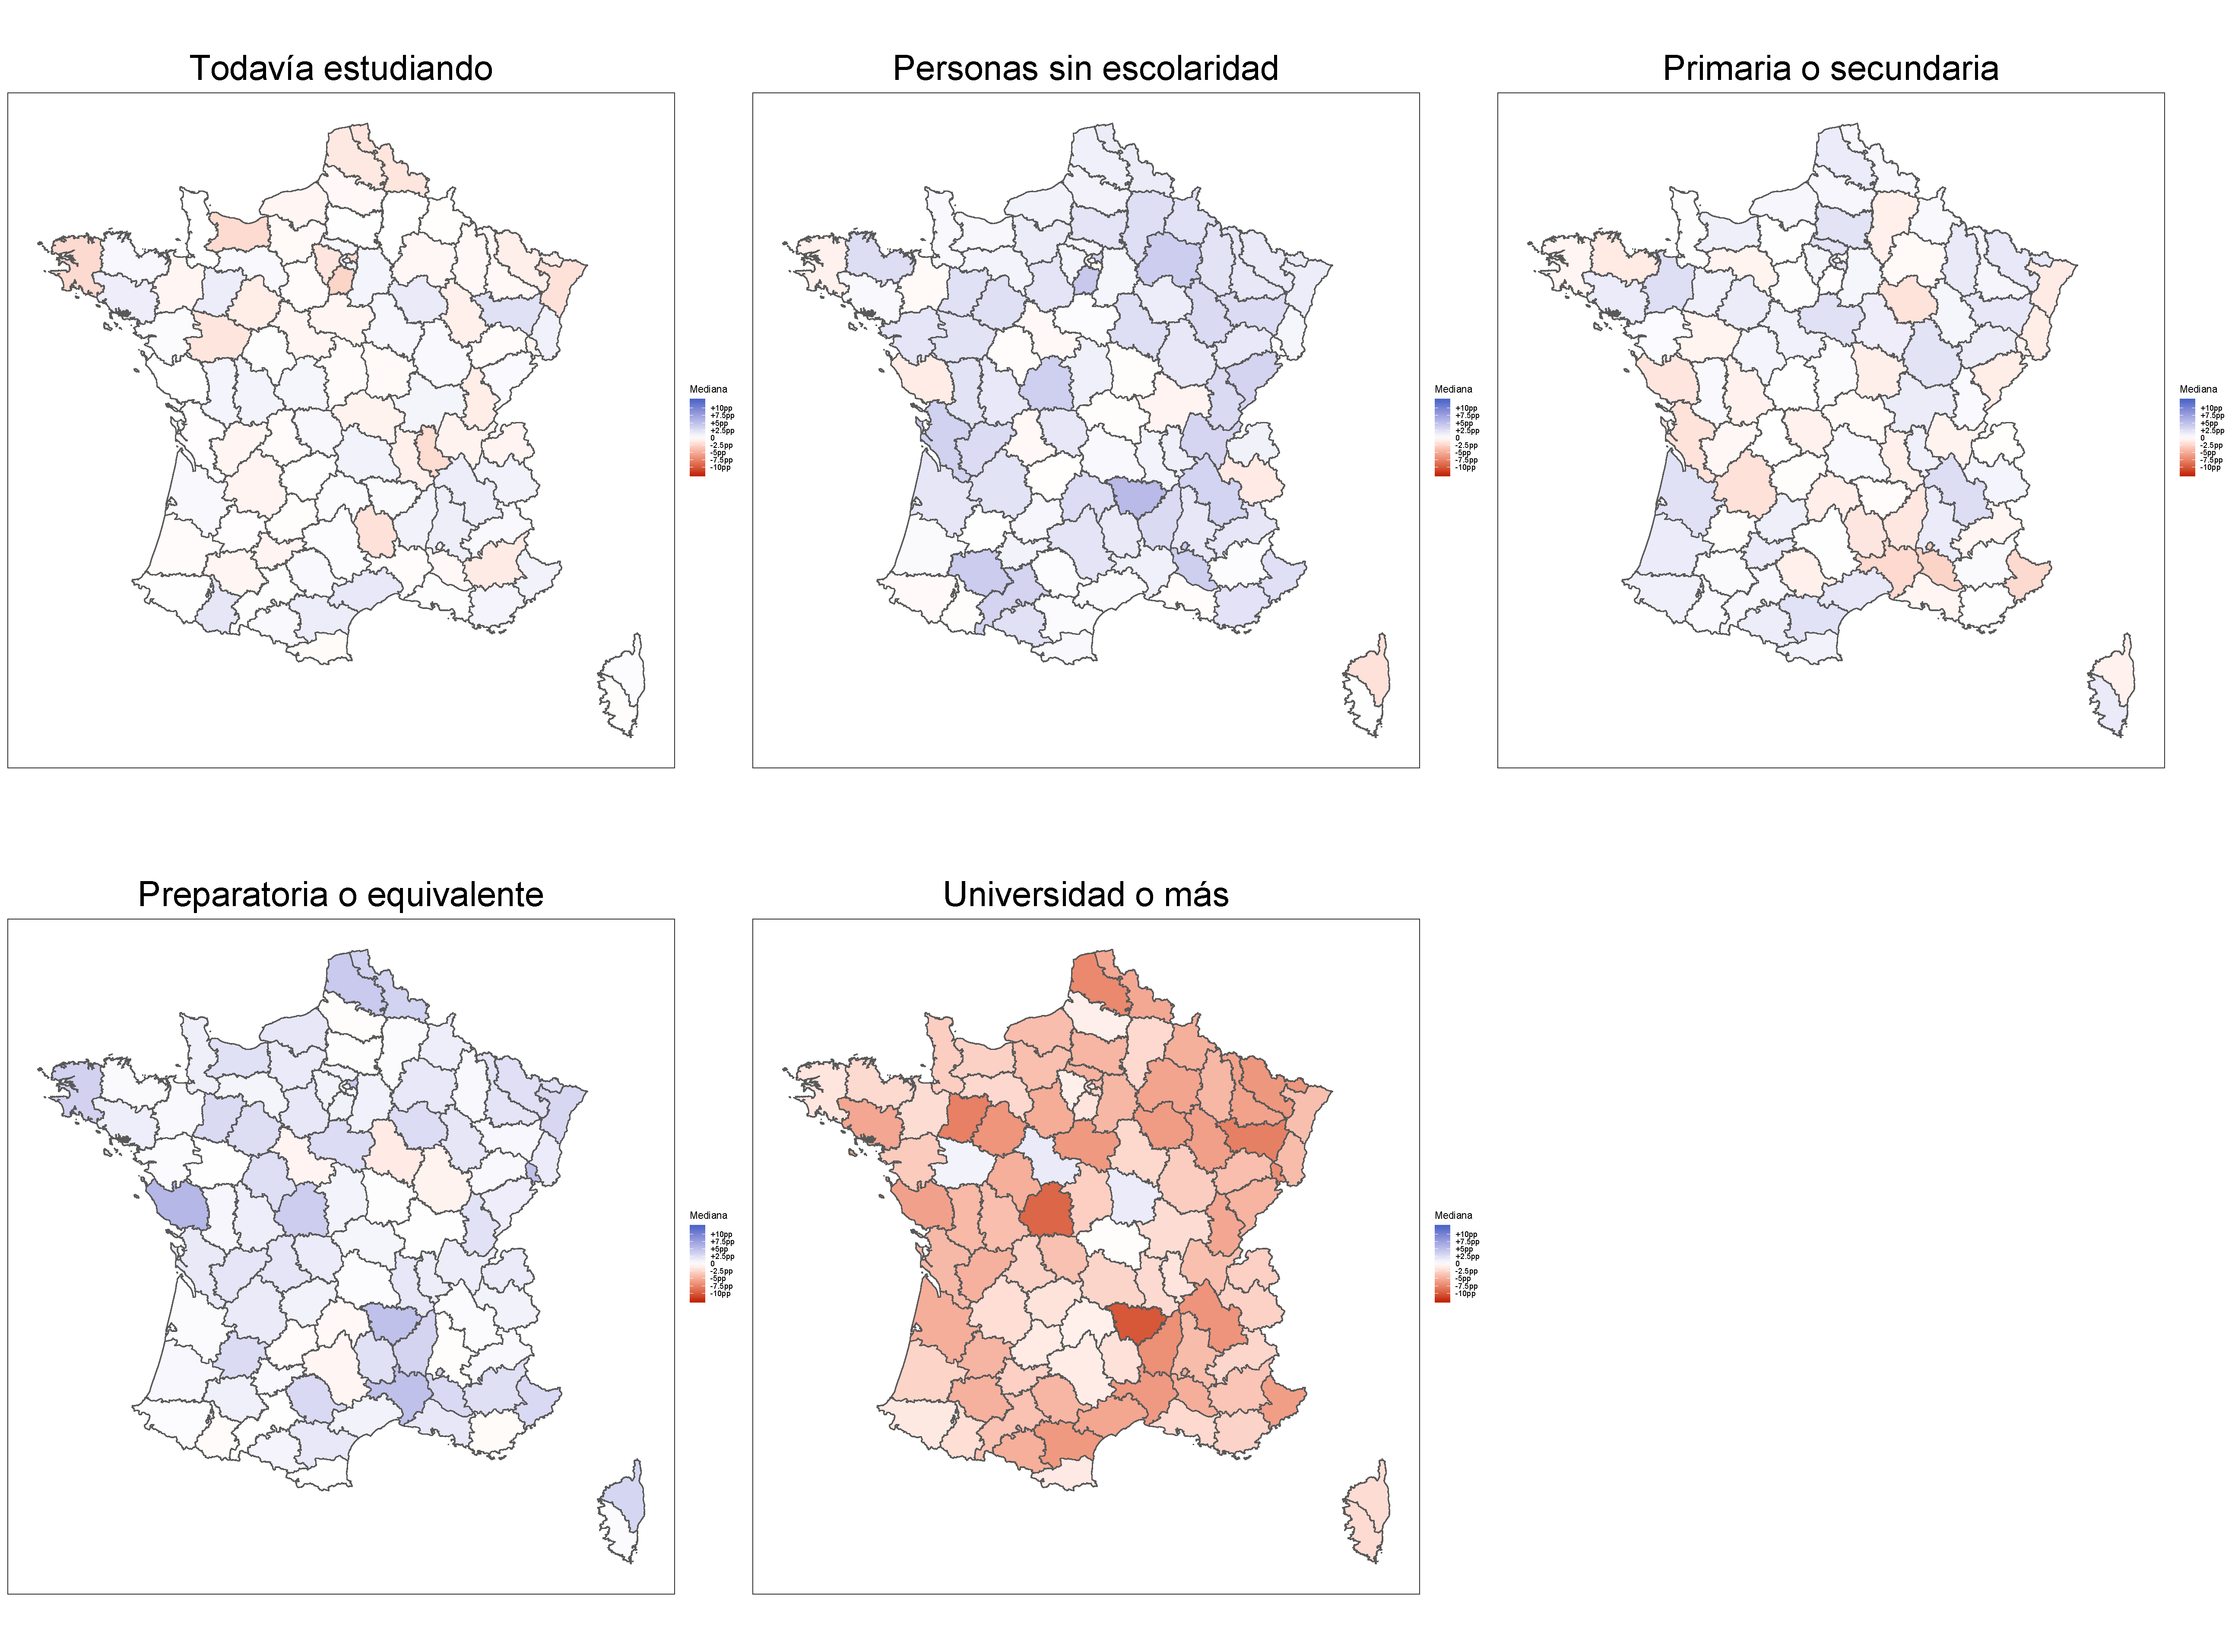
\includegraphics[width = 0.9\textwidth]{Figs/Efectos/Mapa_Efectos_Escolaridad_Modelo_H}
	\caption{Estimaciones puntuales de los efectos de la escolaridad por departamento francés bajo el modelo H. Fuente: elaboración propia con la cartografía de Open Street Map.}
	\label{fig:Mapa_Efectos_Escolaridad}
\end{sidewaysfigure}

Inmediatamente observamos que la categoría universidad o más tiene un efecto negativo en prácticamente todo el hexágono francés. Algunos departamentos tienen magnitudes altas, reflejadas en la intensidad del color. Por el contrario, el aumento en el porcentaje de personas sin escolaridad parece llevar consigo un aumento en las preferencias por Marine Le Pen en la mayoría de departamentos. No obstante, vemos que en Córcega se daría el efecto contrario. En tonos más claros, es decir con una magnitud menor, el porcentaje de personas con escolaridad equivalente a la preparatoria parece también tener un efecto positivo en la afinidad por el FN. Los mapas de las personas que todavía están estudiando y de personas con primaria o secundaria parecen tener efectos mixtos, aunque los segundos se observan más intensos que los primeros.\\

Ahora bien, estos son solo estimadores puntuales. Una de las principales ventajas de los modelos jerárquicos bayesianos es que nos permiten reconocer la variabilidad de los fenómenos bajo estudio así como reportar la incertidumbre sobre ellos de manera más clara. En la \textbf{Figura \ref{fig:Efectos_Escolaridad}} tenemos un resumen de las distribuciones posteriores de los efectos. Para cada categoría observamos los 96 intervalos centrales de probabilidad al 95\% así como la mediana como estimador puntual que ordena los departamentos por categoría. Si el efecto se estima significativo--- es decir que el intervalo al 95\% excluye al 0---, observamos la distribución marcada en rosa o azul dependiendo del sentido de dicho efecto.\\

\begin{sidewaysfigure}
	\centering
	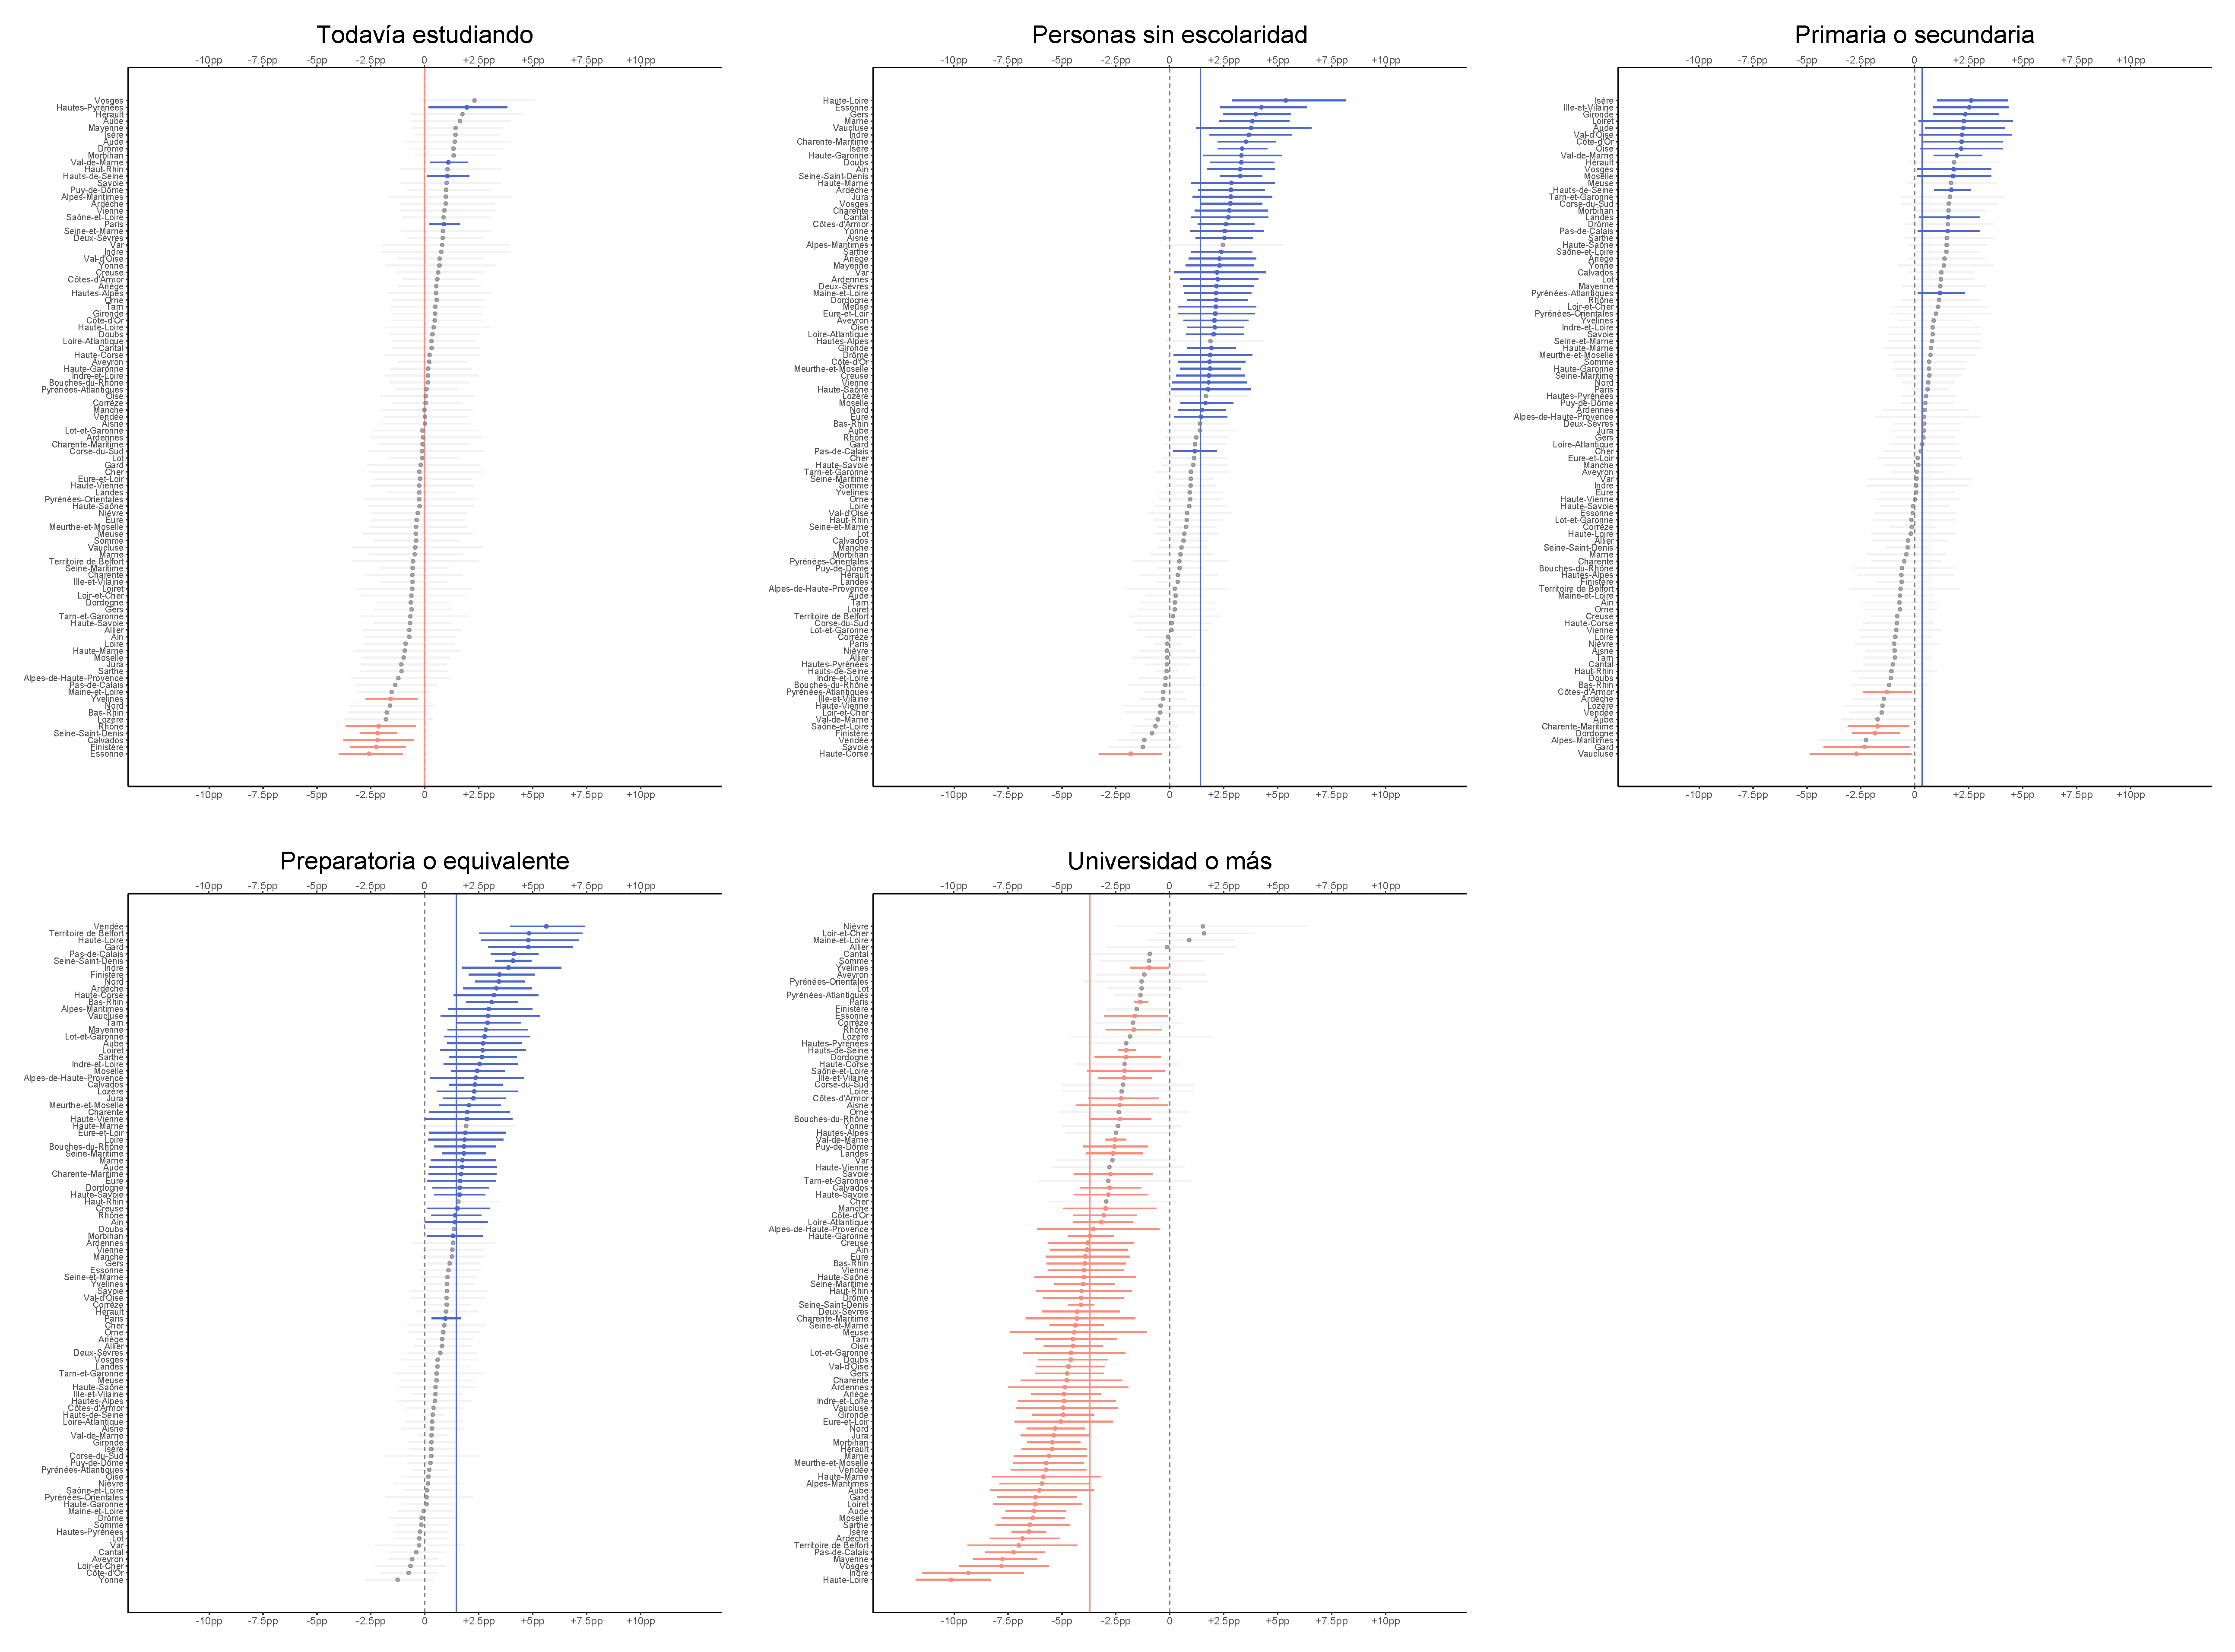
\includegraphics[width = 0.9\textwidth]{Figs/Efectos/Efectos_Escolaridad_Modelo_H}
	\caption{Intervalos centrales de probabilidad al 95\%, 80\% y 50\% para los efectos de la escolaridad por departamento francés bajo el modelo H. Los departamentos se ordenan para cada categoría por magnitud del estimador puntual que es el efecto mediano. Las distribuciones de colores rosa o azul representan que el efecto es significativo al 95\%. Las lineas verticales representan el efecto promedio a través de los departamentos. Fuente: elaboración propia.}
	\label{fig:Efectos_Escolaridad}
\end{sidewaysfigure}

Podemos hacer varias lecturas de este gráfico. En primer lugar confirmamos mediante las líneas verticales que, en general, un aumento en la proporción de personas con estudios universitarios disminuyó la afinidad comunal por Le Pen. De hecho, la mayoría de departamentos tienen efectos significativos; algunos, como Haute-Loire o Indre, incluso cercanos a -10 pp. ¡Esto es un efecto considerable, dado que estamos comparando una comuna promedio con una con 10 pp más de personas con escolaridad universitaria!\\

Por el contrario, el resto de categorías de escolaridad tienen efectos positivos en la afinidad frontista, aunque no todas en la misma magnitud y en todos los departamentos. Confirmamos que para las personas sin escolaridad la mayoría de departamentos tienen un efecto positivo, el más grande de al rededor de 5 puntos porcentuales por 10 de aumento en esta categoría poblacional. Pero también vemos que, aunque hay incertidumbre reflejada en la longitud del intervalo, en Haute-Corse el efecto es el contrario, aproximadamente de -1.8 pp.\\ 

La categoría de preparatoria tiene muchos departamentos con efectos significativos positivos y ninguno con efecto significativo negativo. Pero aquí también vemos al modelado jerárquico en acción. Aunque hayan muchos departamentos significativos, la incertidumbre es distinta a través de ellos. Comparemos por ejemplo las longitudes de los intervalos de los 7 departamentos con mayor efecto mediano. También podemos ver en el caso de las personas que todavía estudian que pueden existir efectos con un estimador puntual mayor al de otros, pero que no son significativos.\\

\begin{sidewaysfigure}
	\centering
	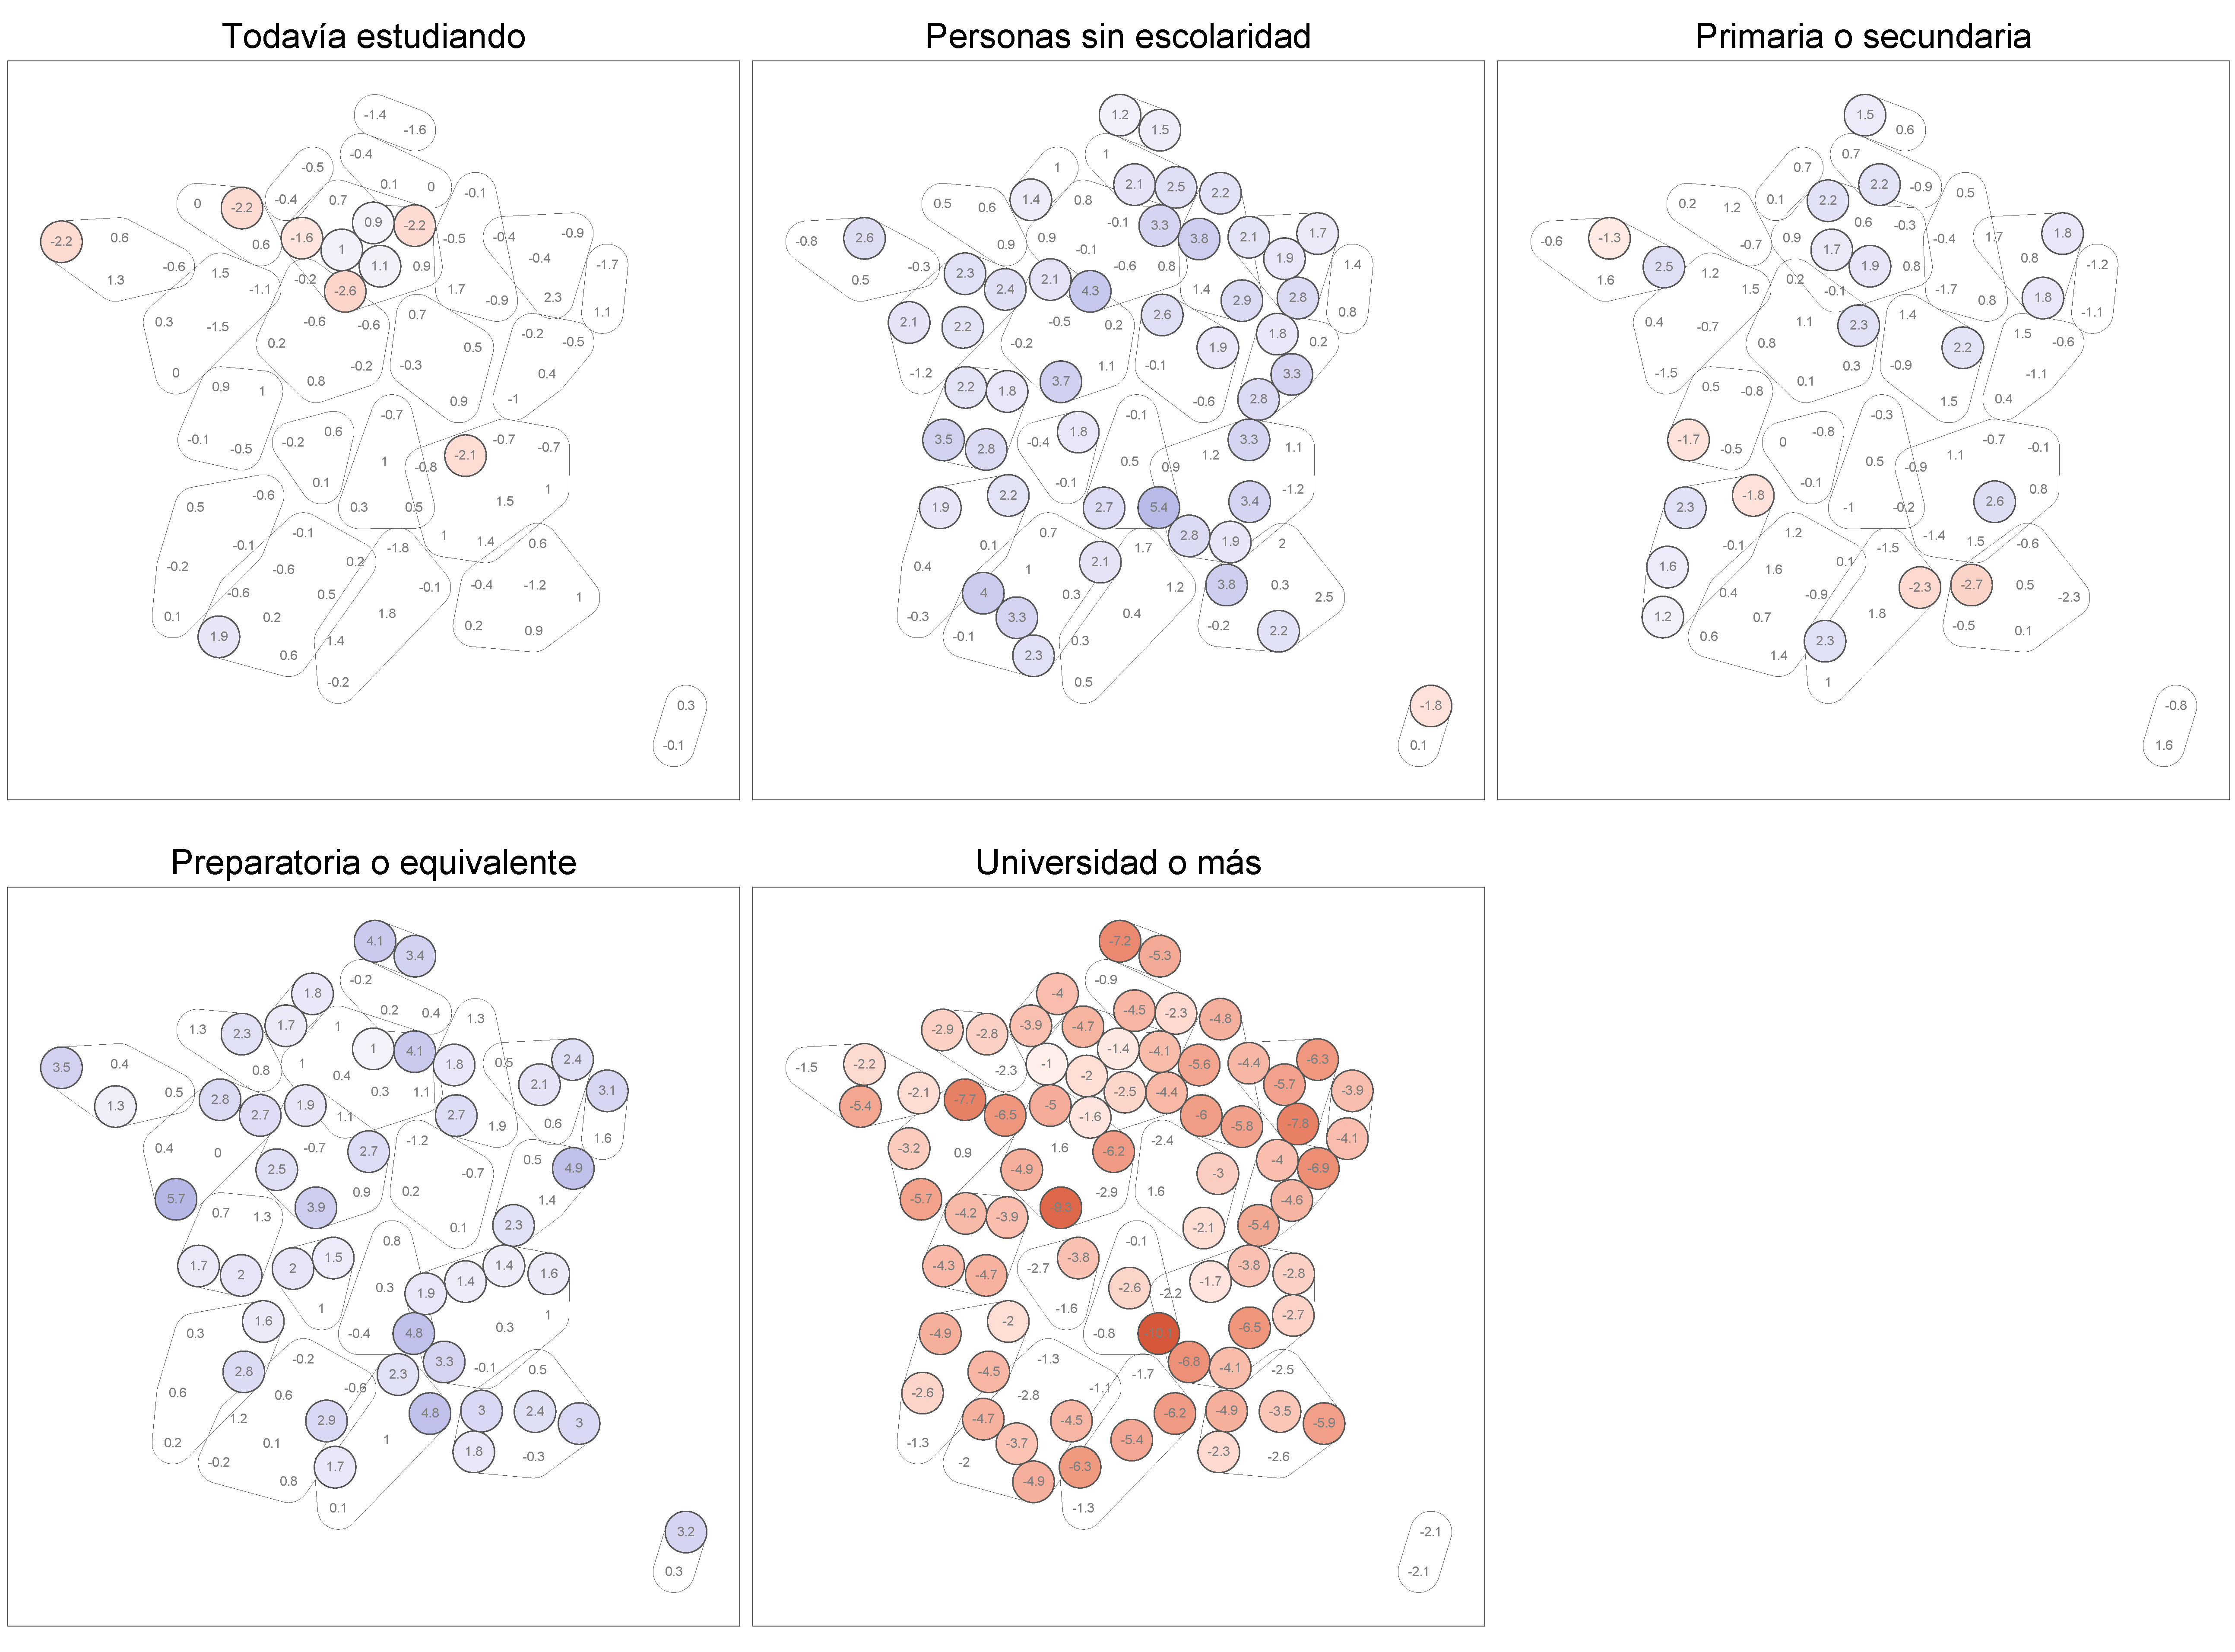
\includegraphics[width = 0.9\textwidth]{Figs/Efectos/Dorling_Efectos_Escolaridad_Modelo_H}
	\caption{Estimaciones puntuales de los efectos de la escolaridad por departamento francés bajo el modelo H, solo se colorean los efectos significativos. Fuente: elaboración propia.}
	\label{fig:Dorling_Efectos_Escolaridad}
\end{sidewaysfigure}

Tomando en cuenta entonces el carácter de significancia o no de un efecto, podemos modificar el mapa de la \textbf{Figura \ref{fig:Mapa_Efectos_Escolaridad}} y convertirlo en el dorling de la \textbf{Figura \ref{fig:Dorling_Efectos_Escolaridad}}. En este último, solo tienen color los departamentos con efecto significativo, aunque reporto los efectos esperados en todos los departamentos. Aquí identificamos que las únicas zonas donde el efecto de los universitarios no parece ser significativo es en departamentos más rurales como el llamado \textit{Massif Central}. Por el contrario, si en general el porcentaje de personas que todavía estudian no parecía ser tan importante, aquí observamos que sus efectos significativos se concentran en la región de Île de France. 

\section{Categorías socioprofesionales}

La segunda variable a considerar son las categorías socioprofesionales. Como indicaba en la revisión de literatura esta es probablemente la variable más utilizada en el estudio de la sociología electoral francesa. A pesar de ello, los mapas de la \textbf{Figura \ref{fig:Mapa_Efectos_Cat_Socioprof}} aparecen descolorados para la mayoría de categorías, indicando efectos muy pequeños. Resalta inmediatamente un departamento al noreste francés coloreado con un azul más intenso en el panel de obreros, la que es la categoría que parece tener una mayor asociación positiva con las preferencias por Marine Le Pen. Esto refuerza las hipótesis sobre \textit{gaucho-lépénisme} discutidas en la primera parte de este trabajo. Llama particularmente la atención la falta de intensidad en los efectos de los artesanos, comerciantes y empresarios, un grupo tradicionalmente asociado al FN. Otro punto interesante es notar que los cuadros y las profesiones intelectuales superiores tienen un efecto negativo, salvo en pocos departamentos que aparecen claramente en azul.\\ 

Al observar los intervalos de los efectos en la \textbf{Figura \ref{fig:Efectos_Cat_Socioprof}}, confirmamos que la mayoría de las categorías tienen efectos muy pequeños de acuerdo a los promedios a través de departamentos observados en las líneas verticales. La única categoría con un efecto promedio mayor parece ser la de los obreros donde Meuse es el departamento con el mayor efecto, de más de 4 puntos porcentuales. Esta también sería la categoría socioprofesional más cercana a un sentimiento de clase lo que podría explicar su mayor homogeneidad nacional frente a otras categorías que, como la investigación de \textcite{MayerMichelat81} ya sugería, pueden cambiar más sus inclinaciones políticas dependiendo del contexto local, reafirmando incluso la influencia que la mayor presencia de obreros tiene en la preferencia electoral de otras categorías.\\ 

\begin{figure}[H]
	\centering
	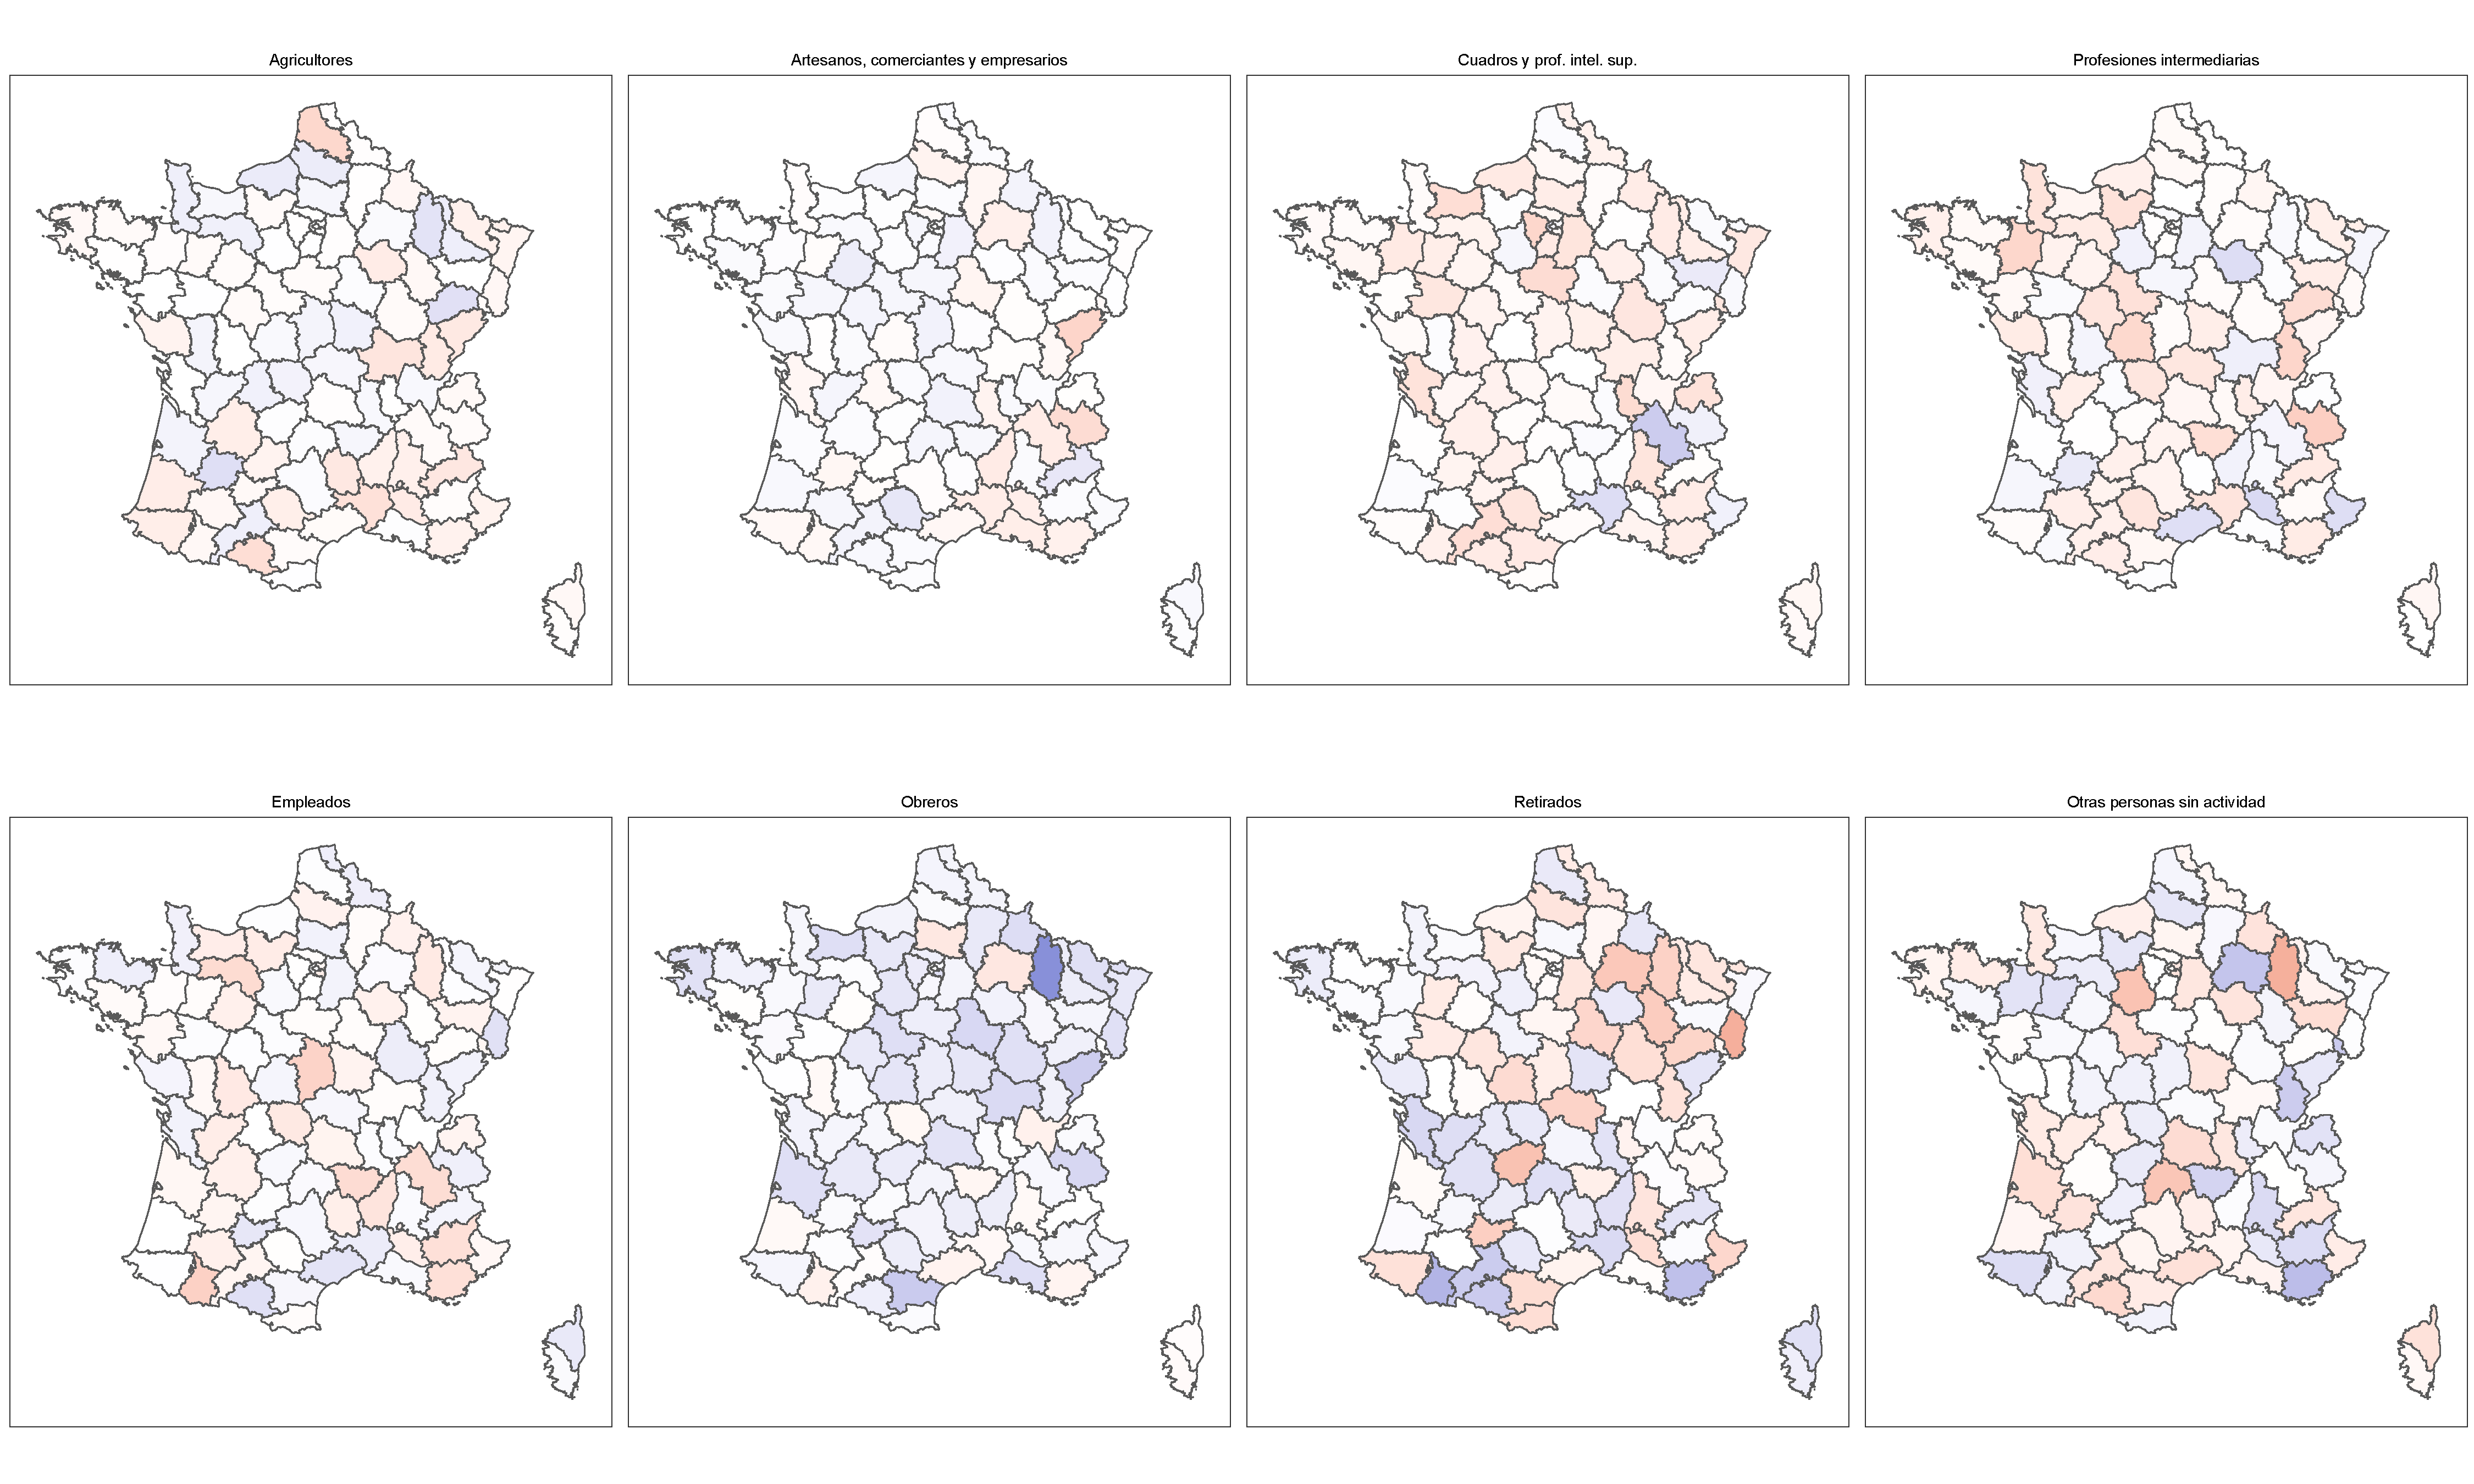
\includegraphics[width = 0.95\textwidth]{Figs/Efectos/Mapa_Efectos_Cat_Socioprof_Modelo_H}
	\caption{Estimaciones puntuales de los efectos de la categoría socioprofesional por departamento francés bajo el modelo H. Fuente: elaboración propia con la cartografía de Open Street Map.}
	\label{fig:Mapa_Efectos_Cat_Socioprof}
\end{figure}

Llama la atención también que para las profesiones intermediarias la mayoría de los efectos significativos son negativos, sin embargo tenemos 4 departamentos con claros efectos positivos y todos en zonas de fortaleza del FN: Vaucluse, Alpes-Maritimes y Hérault en el litoral mediterráneo y Aube en el noreste francés. El caso de los retirados es interesante porque si bien la mayoría de los efectos son nulos, hay algunos significativos tanto positivos como negativos y la gráfica se ve más dispersa.\\ 

Este es un ejemplo donde el modelo jerárquico se asemeja más a un modelo de no agregación o regresiones independientes. Por el contrario, las gráficas en la que las curvas son casi verticales, indicando efectos muy parecidos para todos los departamentos, serían casos más parecidos a los modelos de agregación completa o una sola regresión nacional.\\ 

\begin{sidewaysfigure}
	\centering
	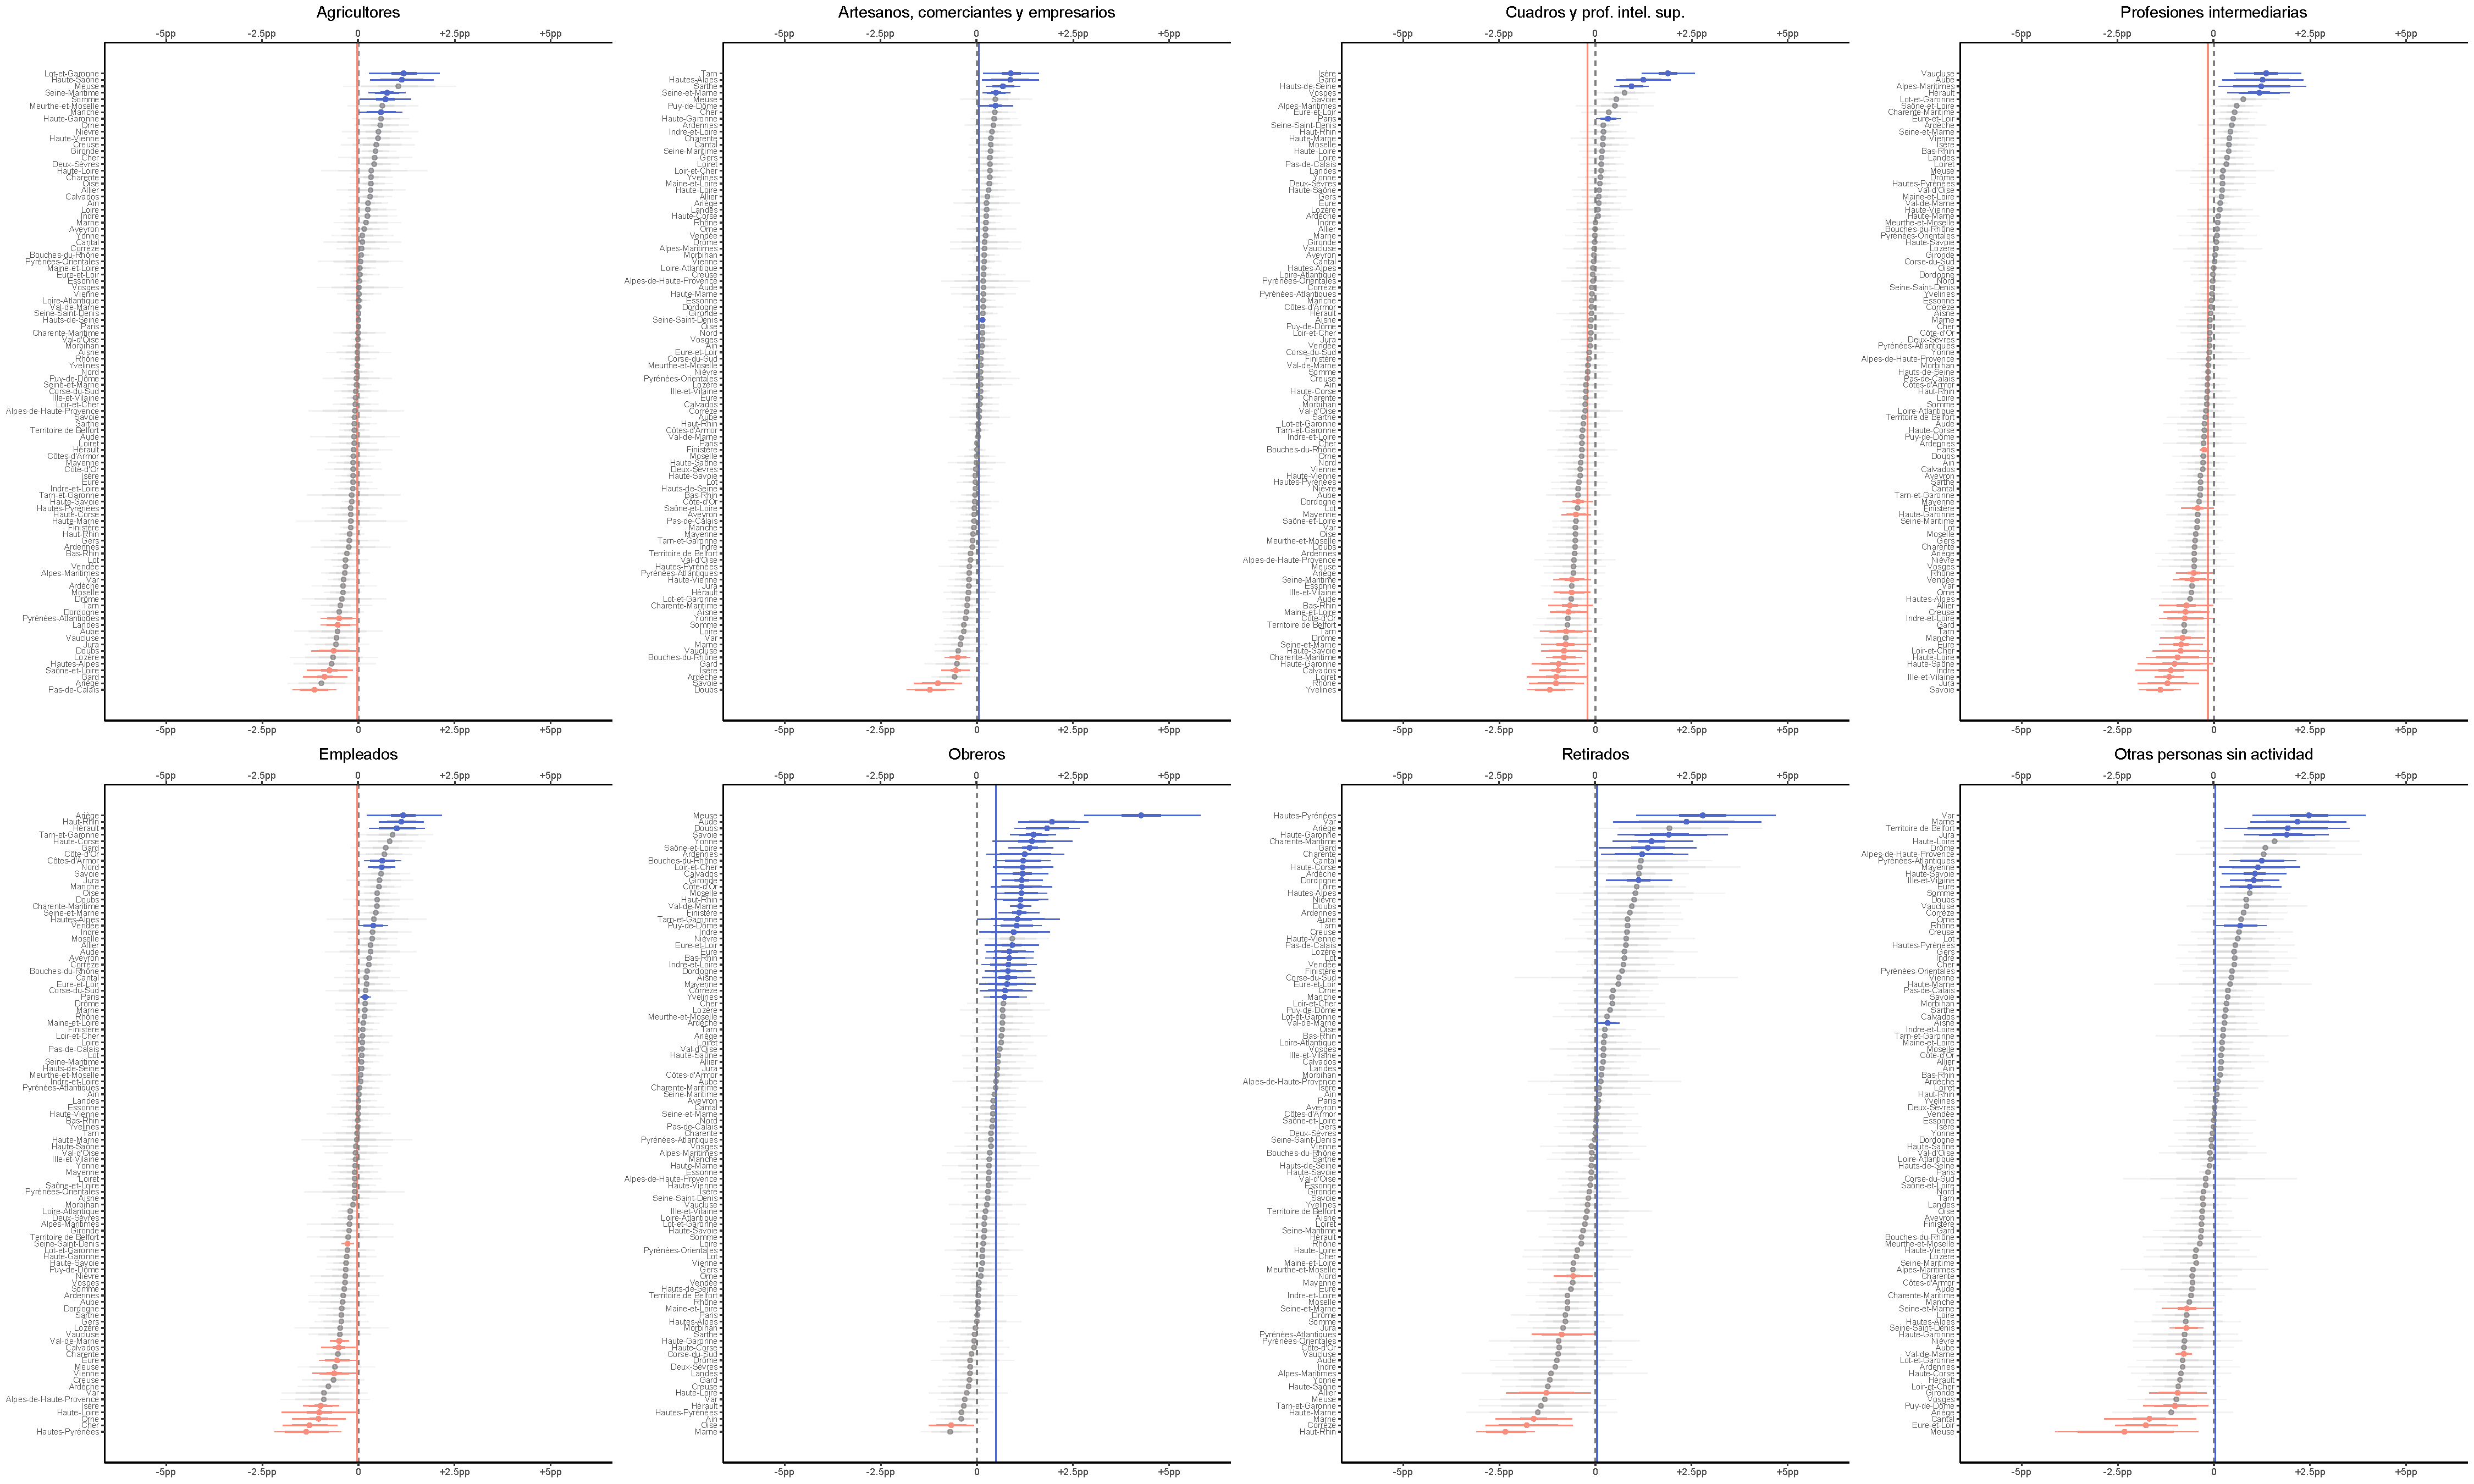
\includegraphics[width = 0.9\textwidth]{Figs/Efectos/Efectos_Cat_Socioprof_Modelo_H}
	\caption{Intervalos centrales de probabilidad al 95\%, 80\% y 50\% para los efectos de la categoría socioprofesional por departamento francés bajo el modelo H. Los departamentos se ordenan para cada categoría por magnitud del estimador puntual que es el efecto mediano. Las distribuciones de colores rosa o azul representan que el efecto es significativo al 95\%. Las lineas verticales representan el efecto promedio a través de los departamentos. Fuente: elaboración propia.}
	\label{fig:Efectos_Cat_Socioprof}
\end{sidewaysfigure}

La geografía de los efectos significativos que se observa en los dorlings de la \textbf{Figura \ref{fig:Dorling_Efectos_Cat_Socioprof}} tiene algunos puntos notables. El norte más industrializado se asocia con mayores efectos de la clase obrera. Vemos la particularidad del litoral mediterráneo en términos de profesiones intermediarias. Quizás sorprende que en París una mayor presencia de cuadros lleva a una mayor preferencia frontista. La explicación podría estar en que los cuadros que logran vivir dentro de París tiendan a ser más cercanos a la derecha, pero esta tendría que ser una hipótesis a explorarse con mayor detalle en otro tipo de estudio. 

\begin{figure}[H]
	\centering
	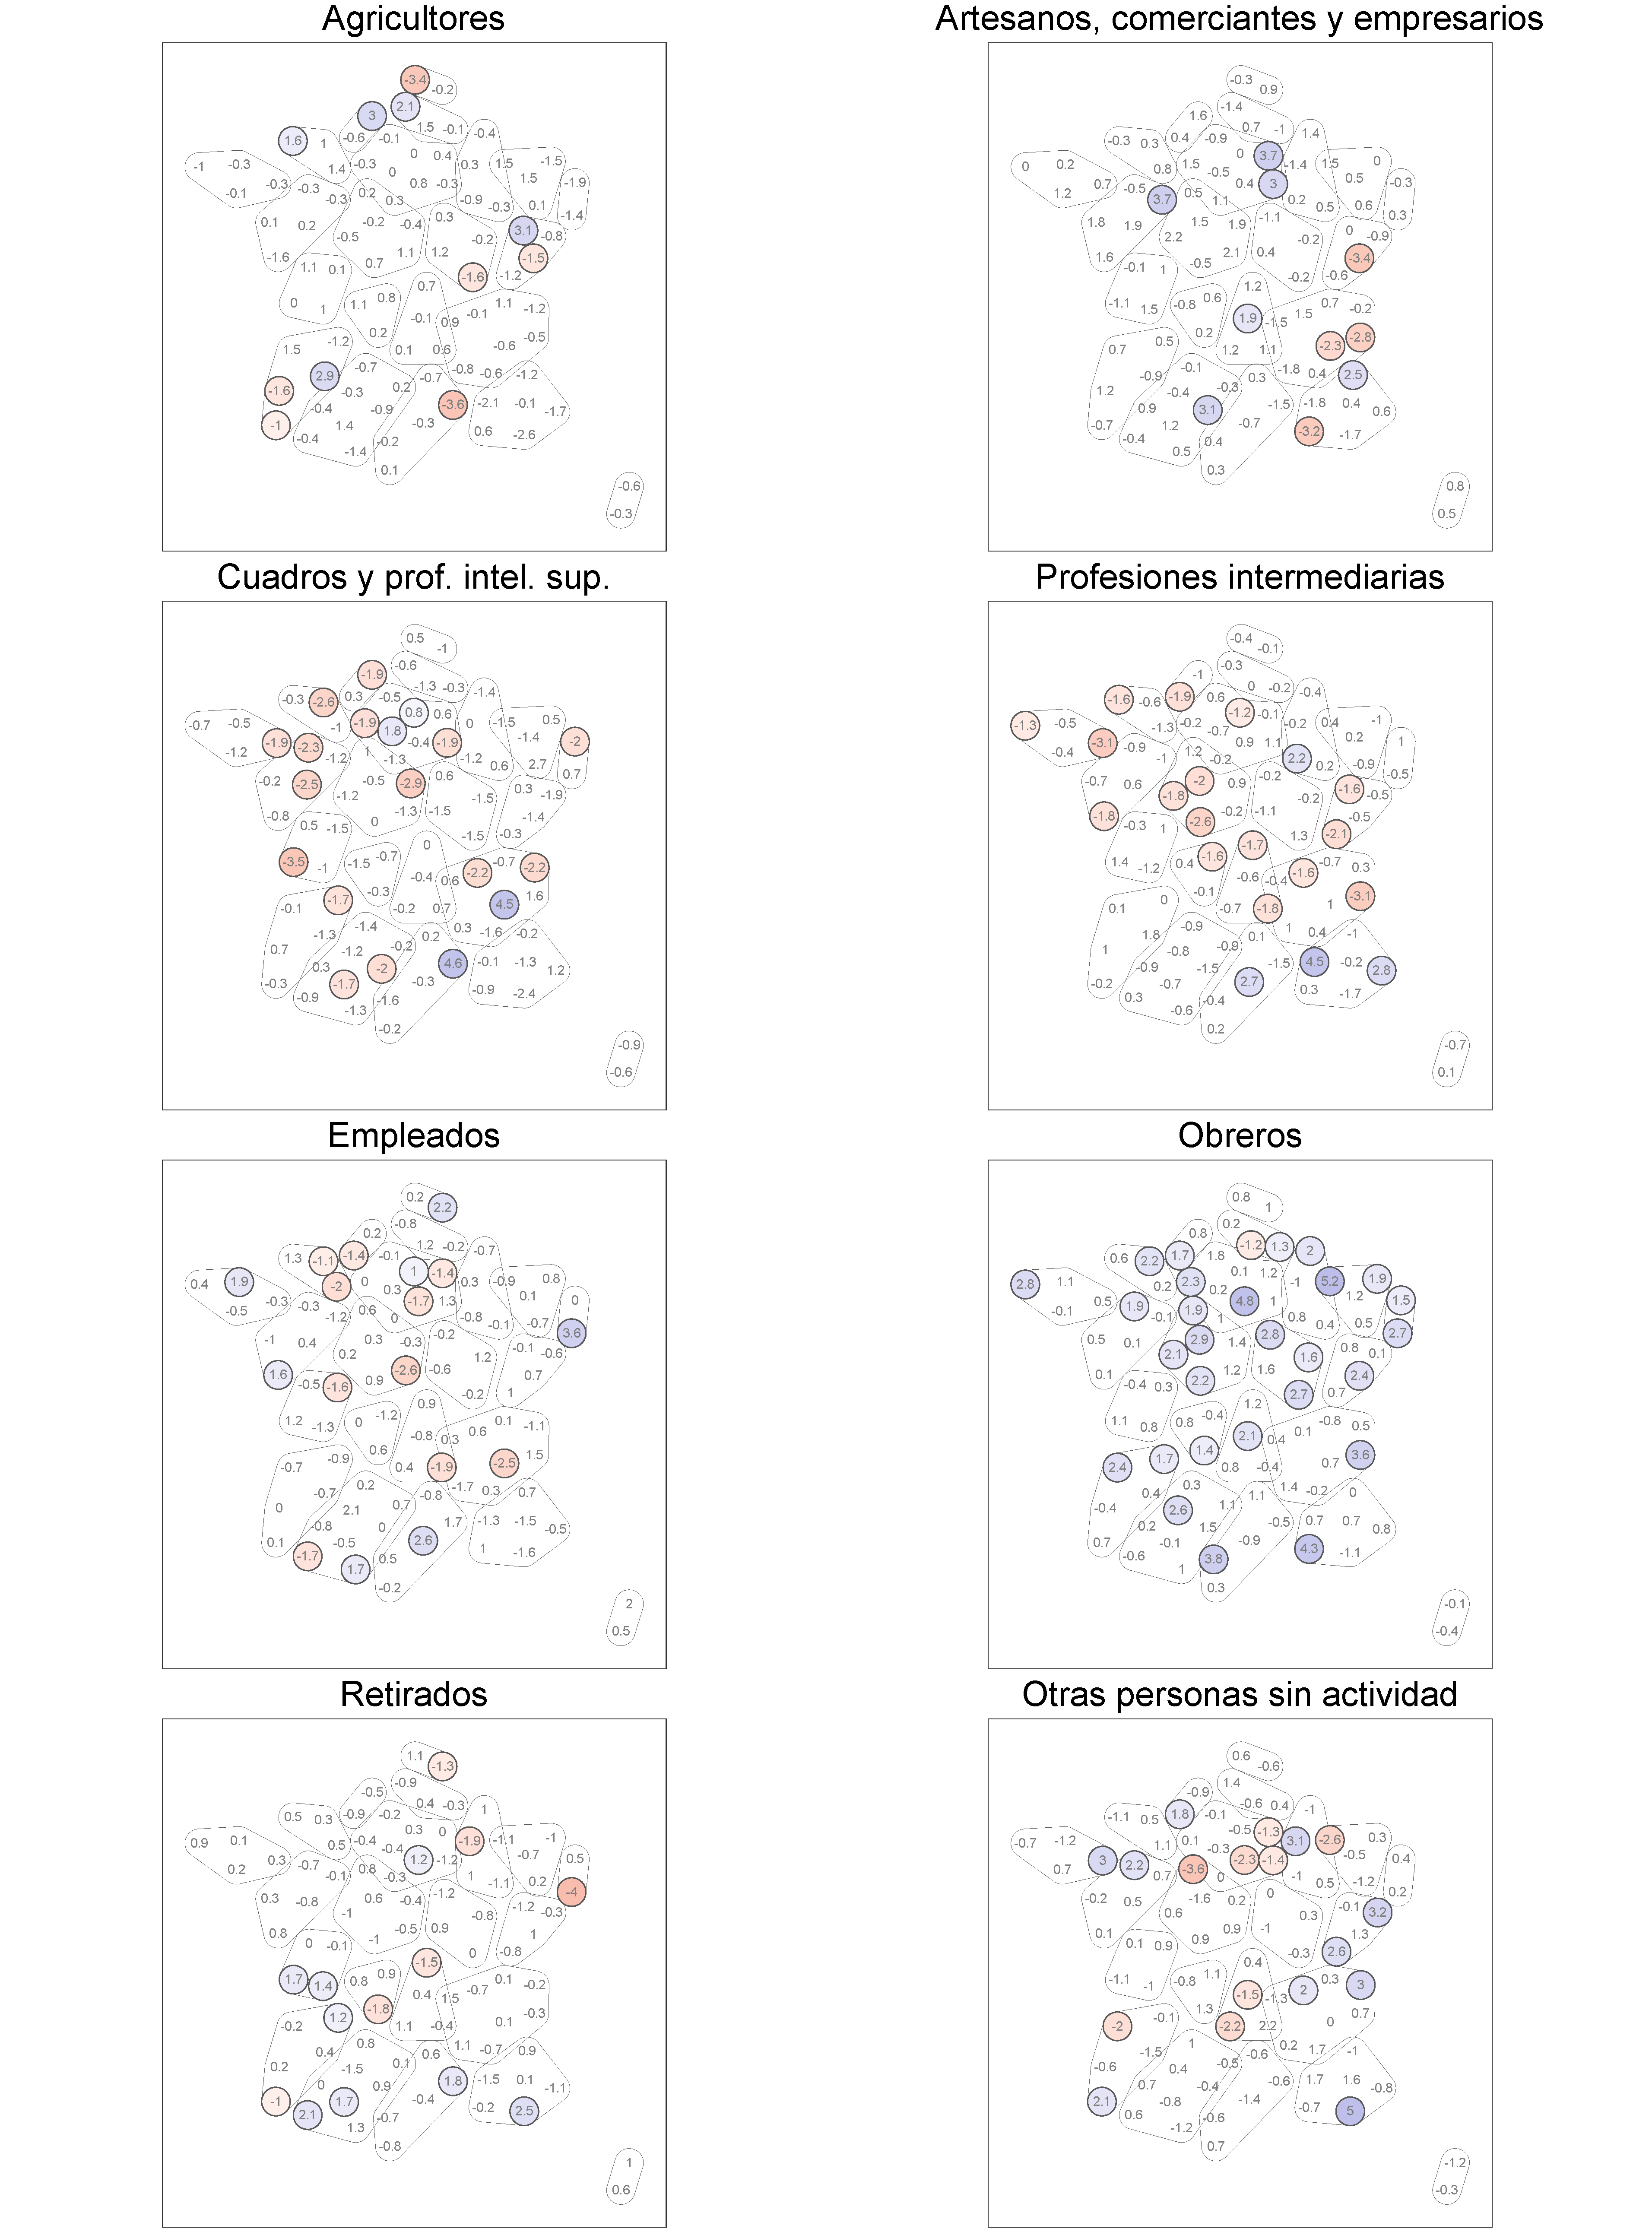
\includegraphics[width = 0.95\textwidth]{Figs/Efectos/Dorling_Efectos_Cat_Socioprof_Modelo_H}
	\caption{Estimaciones puntuales de los efectos de la categoría socioprofesional por departamento francés bajo el modelo H, solo se colorean los efectos significativos. Fuente: elaboración propia.}
	\label{fig:Dorling_Efectos_Cat_Socioprof}
\end{figure}

\section{Edad}

Las explicaciones culturalistas, principalmente las de la escuela de Inglehart, hablan de que las generaciones de edad crecen con ciertos valores que los llevan a tener determinadas posiciones políticas. En este sentido podríamos leer los mapas de la \textbf{Figura \ref{fig:Mapa_Efectos_Edad}} como reflejo de los valores generacionales, lo que explicaría la mayor homogeneidad a través de departamentos frente a las variables antes analizadas. La mayor presencia de adultos mayores estaría relacionada negativamente con el FN porque este grupo de edad tiene una simpatía por la derecha tradicional. Los jóvenes de entre 18 a 24 años, por el contrario, tendrían posiciones políticas contrarias al carácter NAP del FN. La asociación positiva con los menores de edad podría reflejar un efecto cultural en comunas con altas tasas de natalidad o menos avejentadas. Esta hipótesis podría también explicar por qué los departamentos que parecen tener la tendencia contraria son aquelos de Île de France: la mayor presencia de inmigrantes, que normalmente tienen mayores tasas de natalidad, frenaría el voto nativista que los rechaza. Tendríamos que confirmar esto al analizar el efecto que los inmigrantes tuvieron según el modelo.\\

\begin{sidewaysfigure}
	\centering
	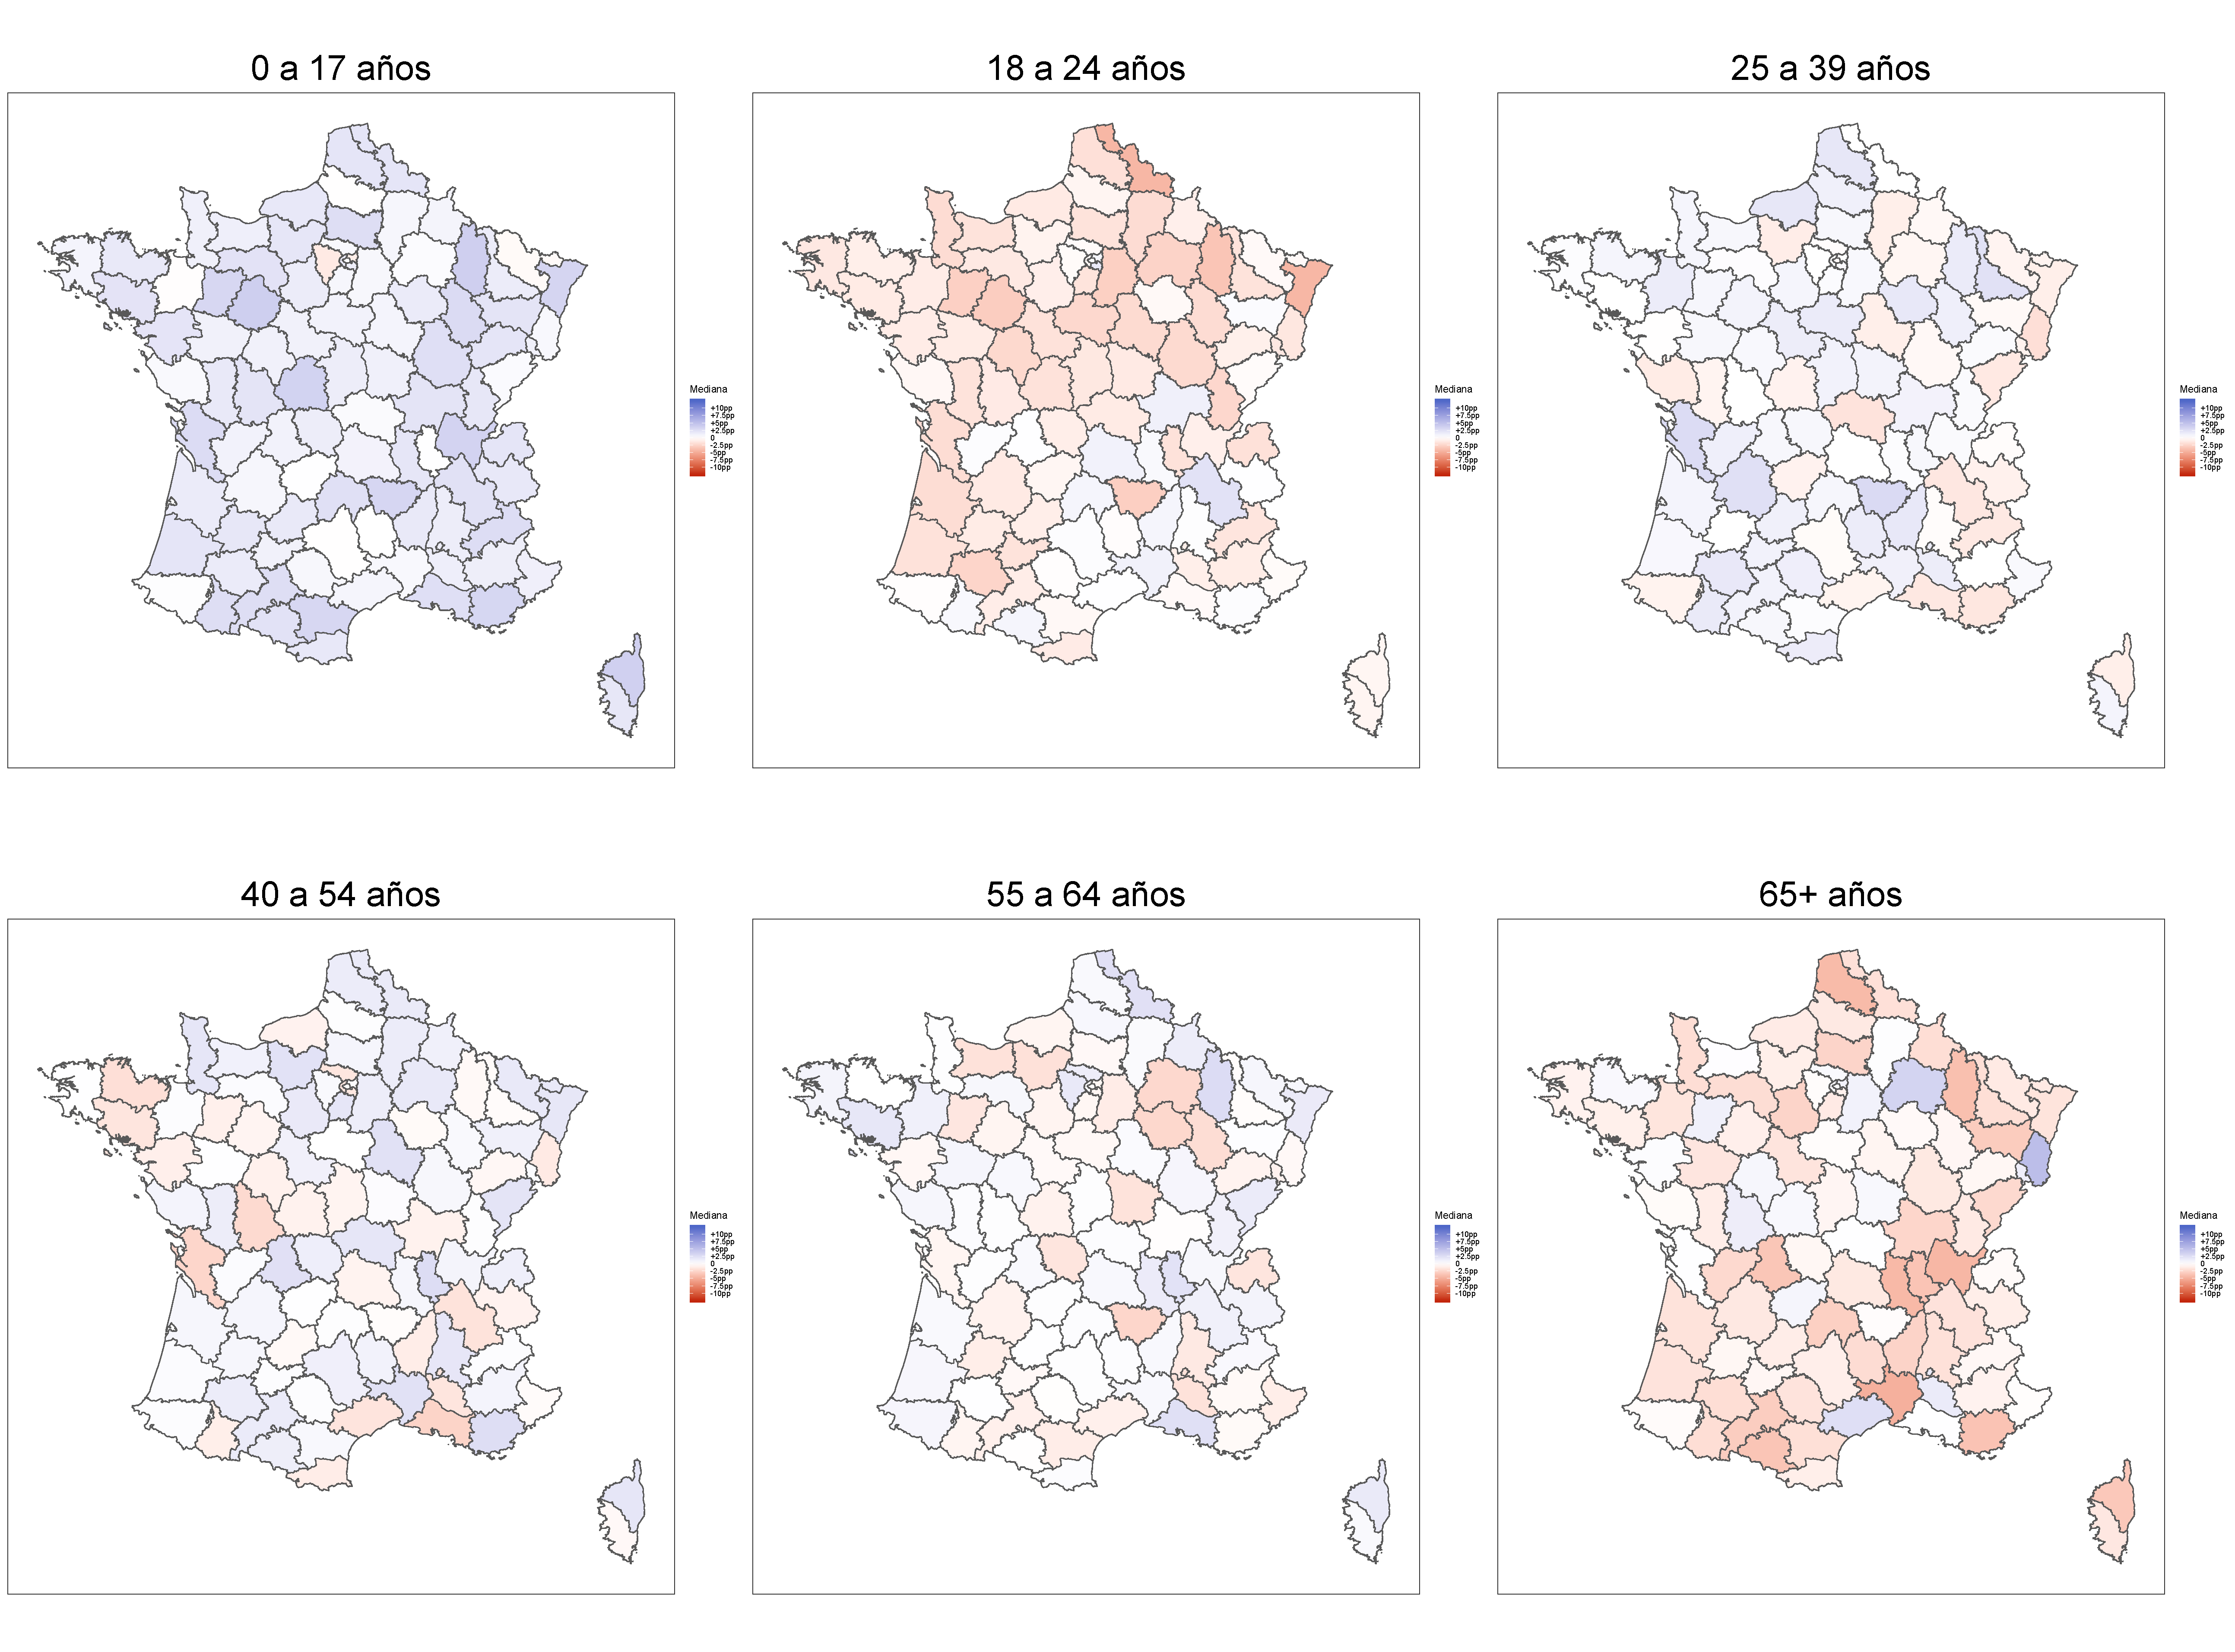
\includegraphics[width = 0.9\textwidth]{Figs/Efectos/Mapa_Efectos_Edad_Modelo_H}
	\caption{Estimaciones puntuales de los efectos del grupo de edad por departamento francés bajo el modelo H. Fuente: elaboración propia con la cartografía de Open Street Map.}
	\label{fig:Mapa_Efectos_Edad}
\end{sidewaysfigure}

Al observar los resúmenes distribucionales confirmamos que los menores de edad y los adultos mayores son los grupos de edad que tienen mayor variabilidad e incertidumbre. En la \textbf{Figura \ref{fig:Efectos_Edad}} vemos que sus intervalos son claramente más largos que los del resto de categorías. De nueva cuenta, modelar mediante una estrategia multinivel tiene la ventaja de permitir que los datos determinen el nivel de agrupamiento necesario sin que el estadístico force a que deba ser total, con una sola regresión, o nulo via regresiones independientes. Observando los dorlings de la \textbf{Figura \ref{fig:Dorling_Efectos_Edad}} vemos que los efectos significativos negativos del grupo de 18 a 24 años se ubican tanto al oeste francés como en el norte. Por otro lado, los mayores de 65 años parecen tener una mayor influencia en el sur del hexágono.

\begin{sidewaysfigure}
	\centering
	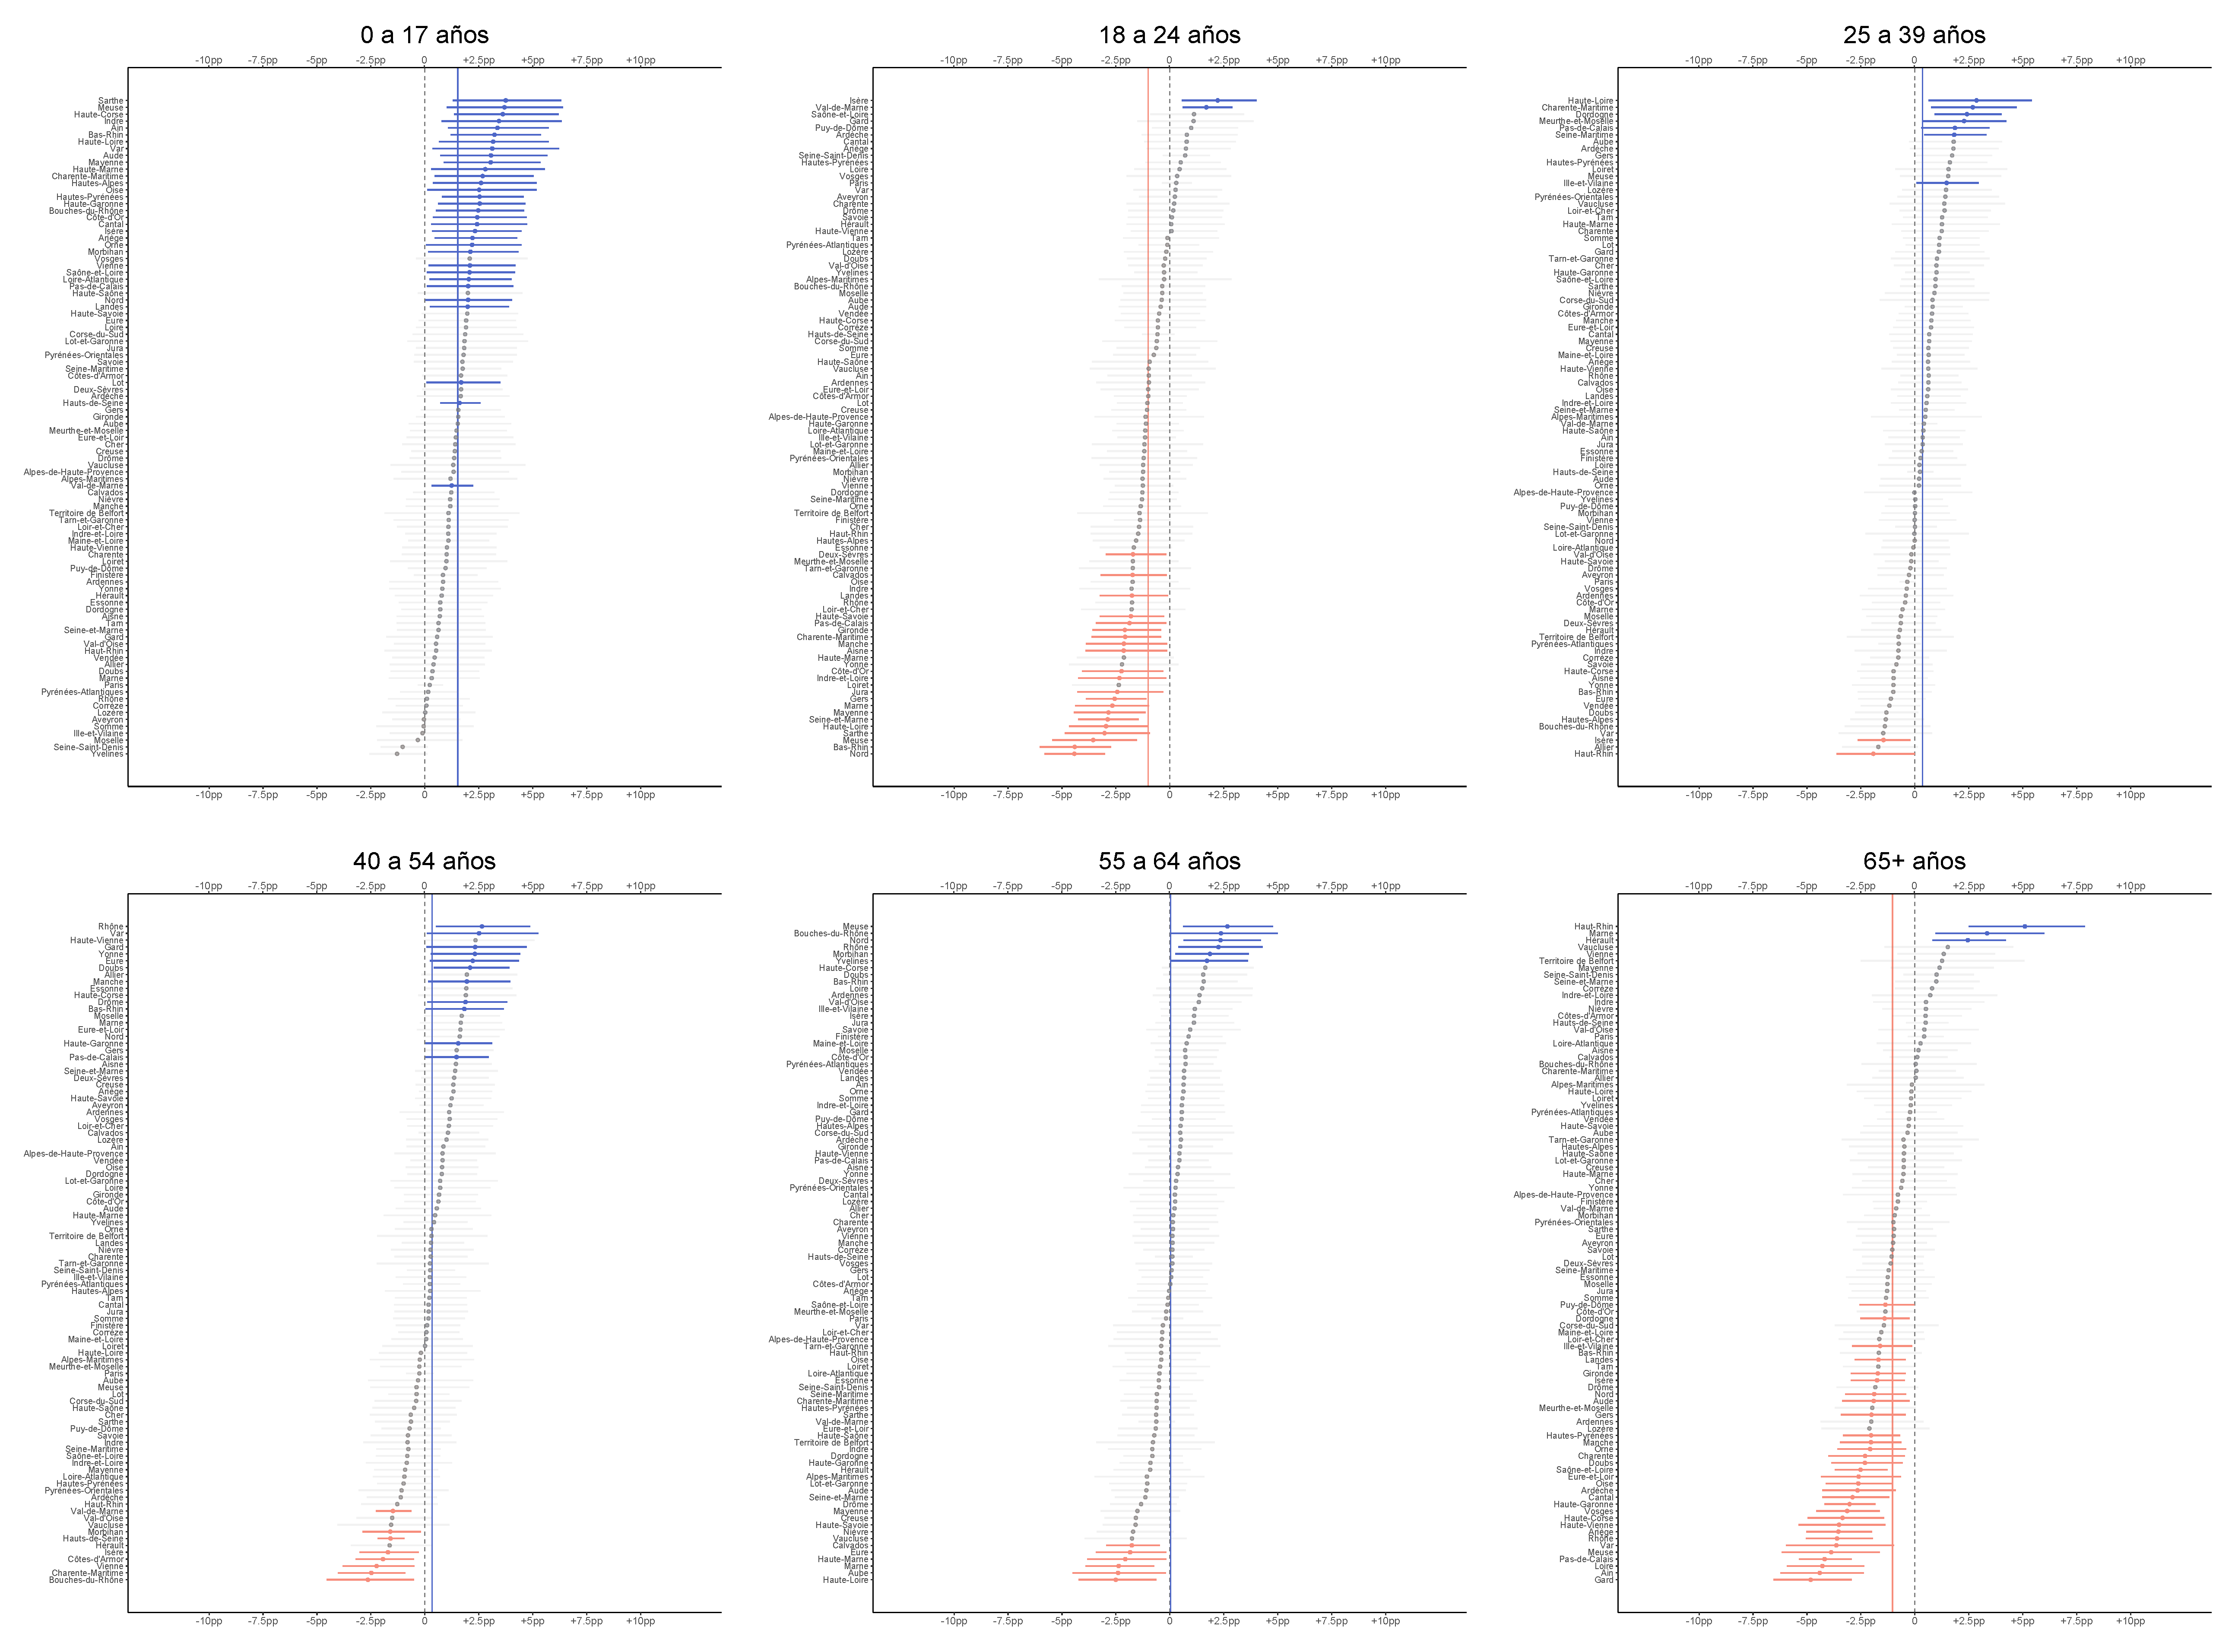
\includegraphics[width = 0.9\textwidth]{Figs/Efectos/Efectos_Edad_Modelo_H}
	\caption{Intervalos centrales de probabilidad al 95\%, 80\% y 50\% para los efectos del grupo de edad por departamento francés bajo el modelo H. Los departamentos se ordenan para cada categoría por magnitud del estimador puntual que es el efecto mediano. Las distribuciones de colores rosa o azul representan que el efecto es significativo al 95\%. Las lineas verticales representan el efecto promedio a través de los departamentos. Fuente: elaboración propia.}
	\label{fig:Efectos_Edad}
\end{sidewaysfigure}

\begin{sidewaysfigure}
	\centering
	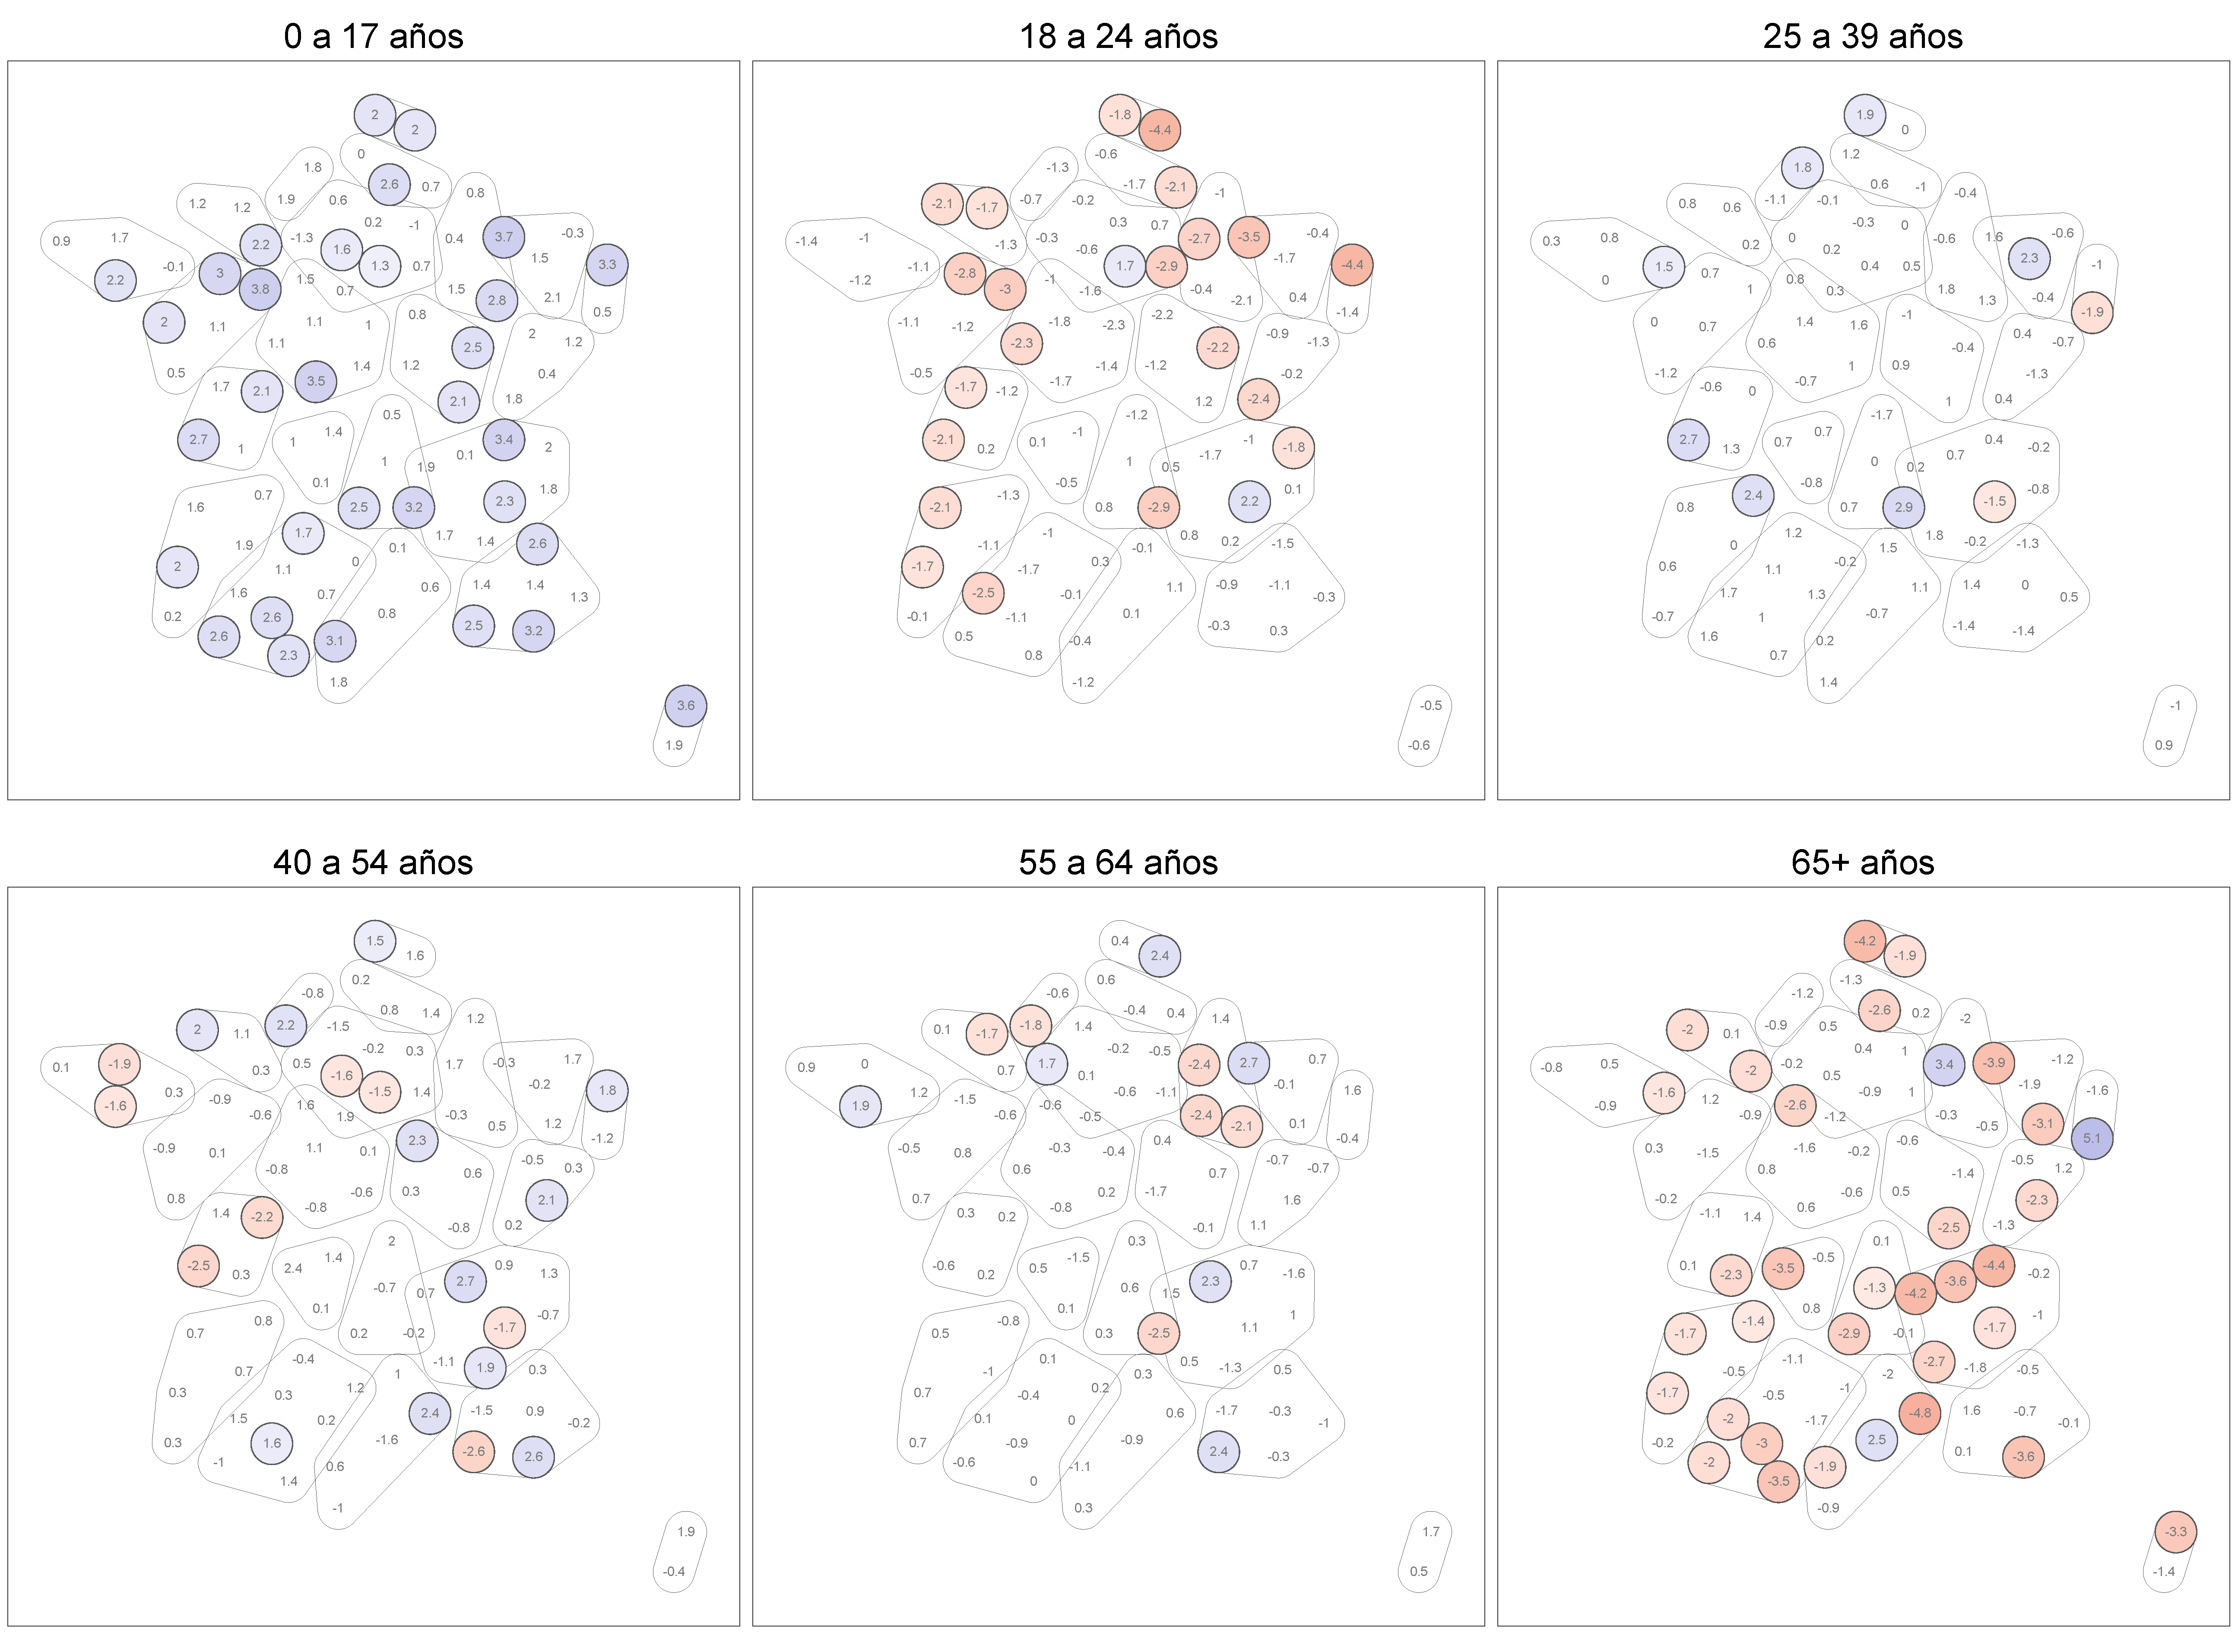
\includegraphics[width = 0.9\textwidth]{Figs/Efectos/Dorling_Efectos_Edad_Modelo_H}
	\caption{Estimaciones puntuales de los efectos del grupo de edad por departamento francés bajo el modelo H, solo se colorean los efectos significativos. Fuente: elaboración propia.}
	\label{fig:Dorling_Efectos_Edad}
\end{sidewaysfigure}

\section{Categorías dicotómicas}

Finalmente, podemos analizar los mapas de las variables dicotómicas, es decir las que tienen solo dos categorías: Sexo, Condición migratoria y (des)ocupaciones. En la \textbf{Figura \ref{fig:Mapa_Efectos_Dicotom}} vemos que la mayor presencia de inmigrantes como de mujeres parece inhibir el voto frontista. Por el contrario, las variables de desempleo no reflejan una geografía muy clara pero sí con efectos en ambos sentidos. Al observar los intervalos de la \textbf{Figura \ref{fig:Efectos_Dicotom}} para estas categorías, nos damos cuenta que existe mucha incertidumbre en las estimaciones, salvo en la del desempleo juvenil. Esto parece continuar confirmándonos que esta no resulta ser la variable con mayor poder explicativo, al menos en términos de configuraciones sociales de las comunas.\\ 

\begin{sidewaysfigure}
	\centering
	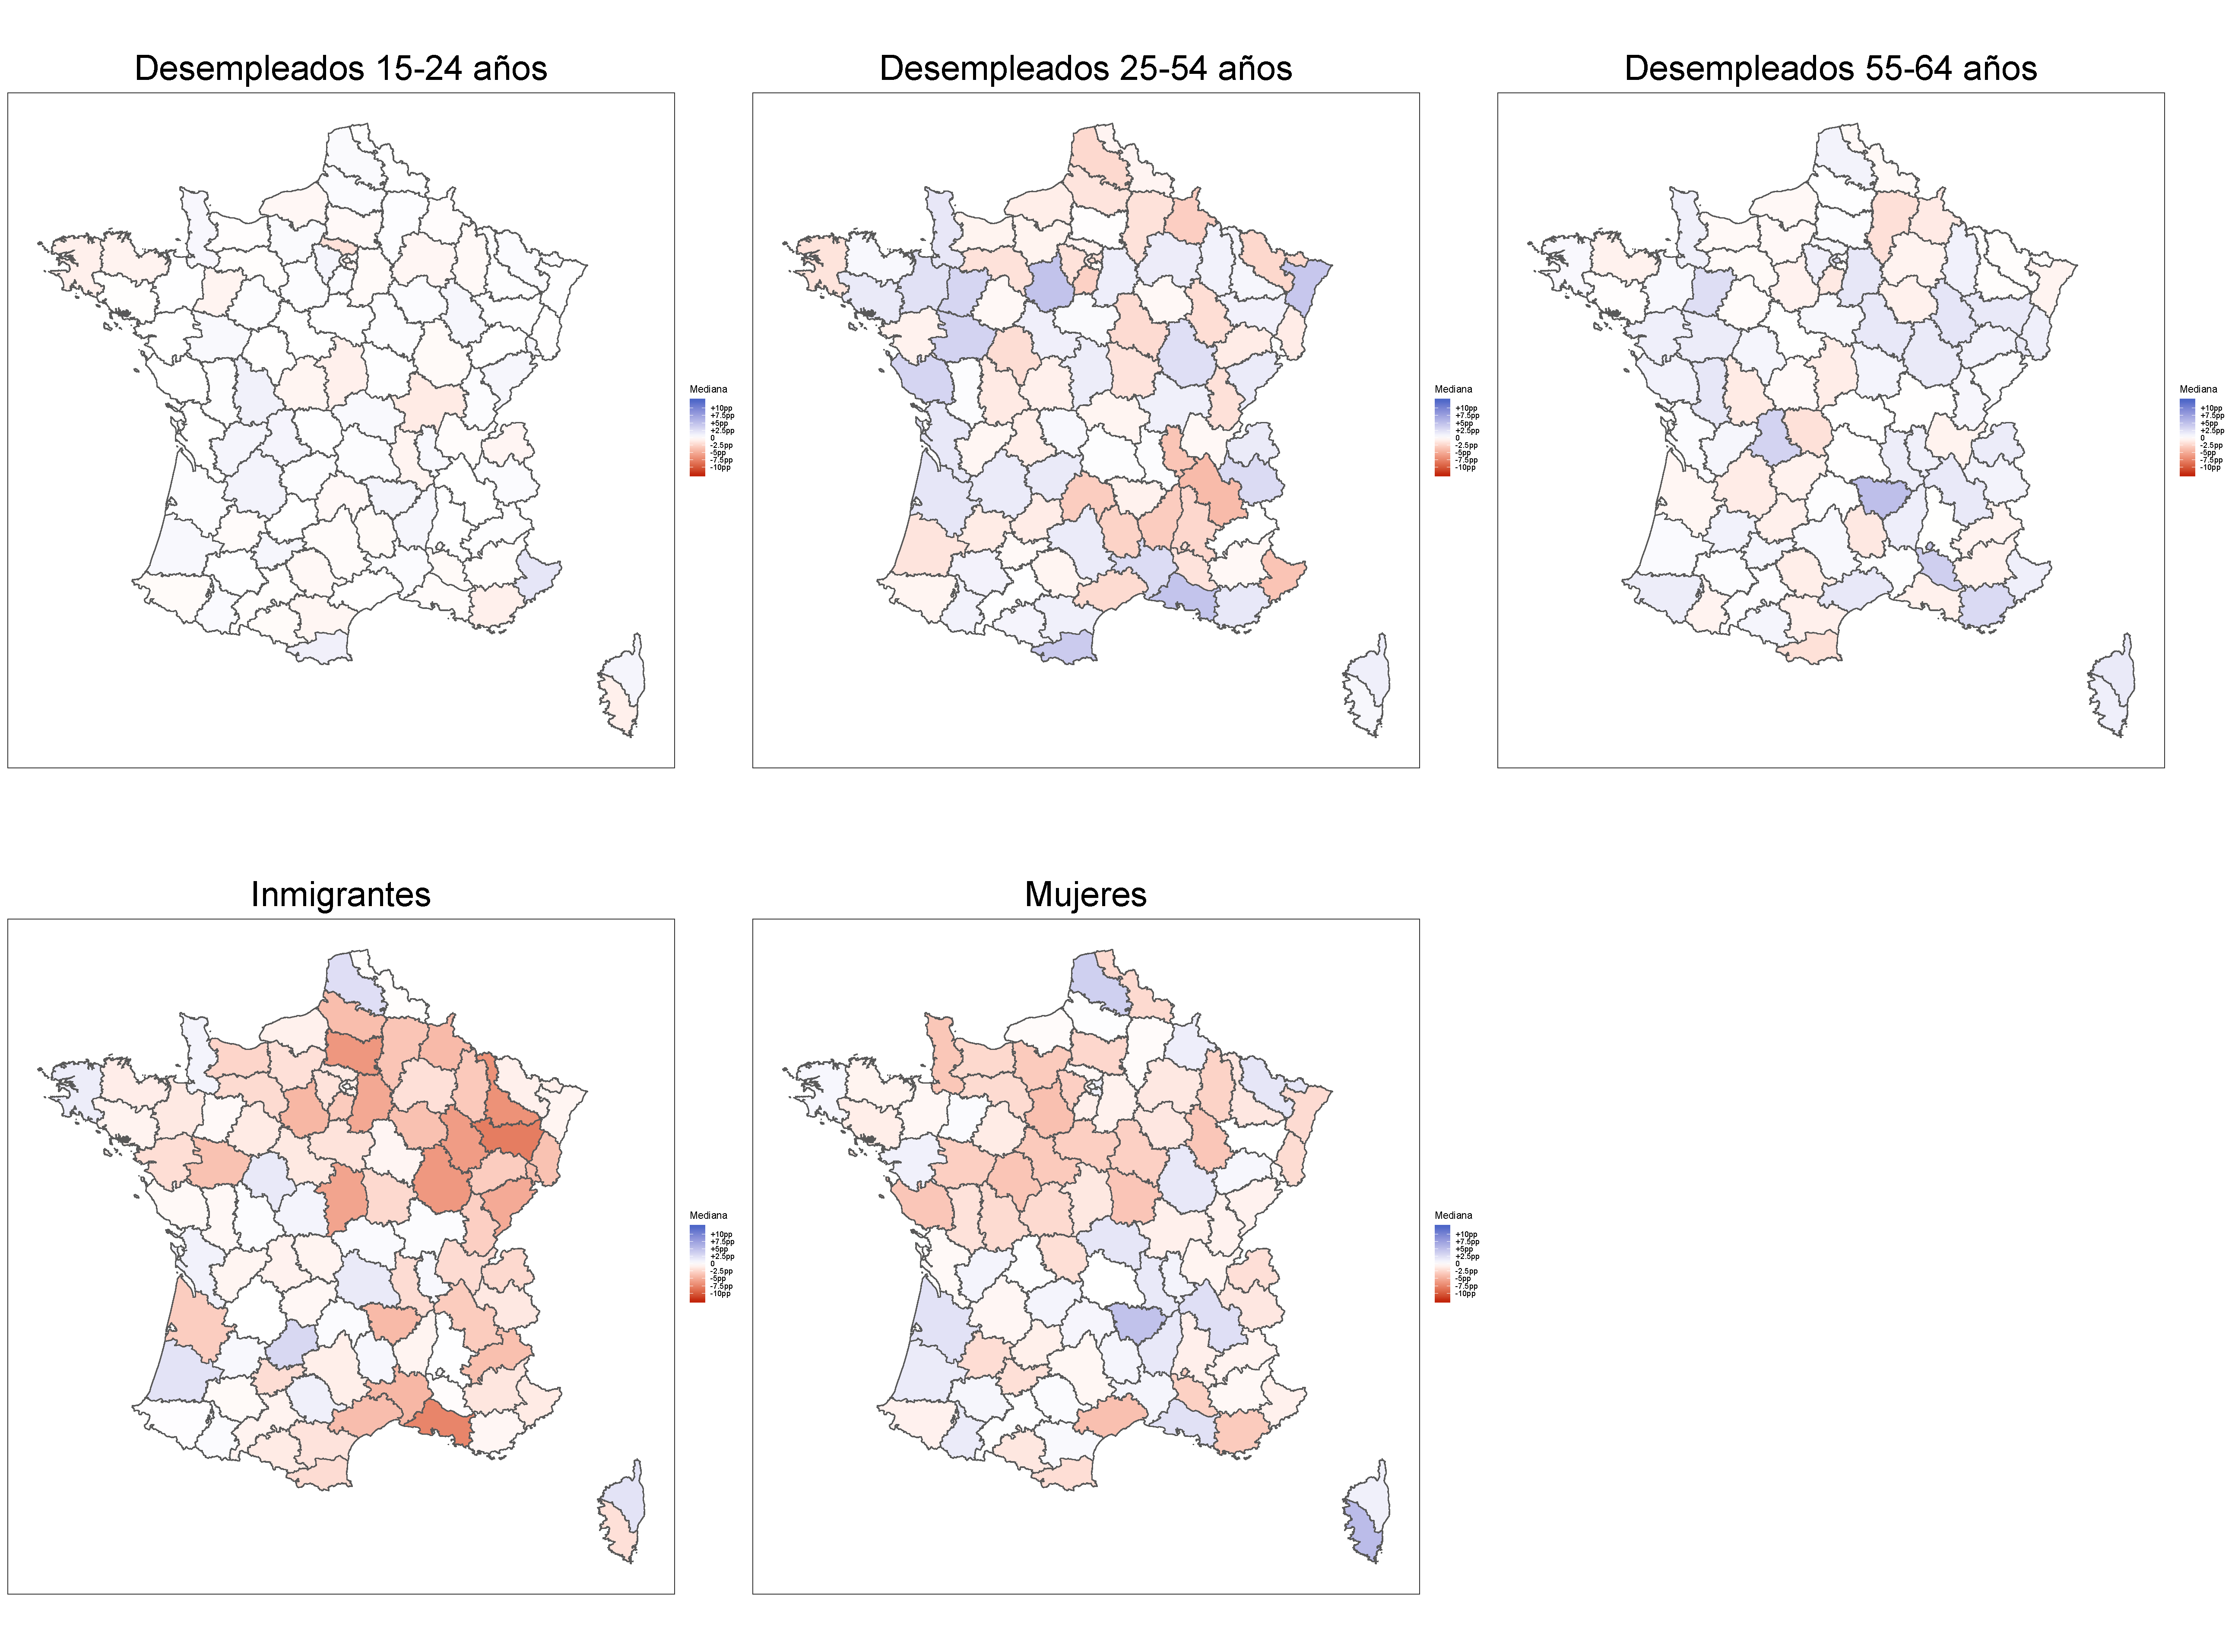
\includegraphics[width = 0.9\textwidth]{Figs/Efectos/Mapa_Efectos_Dicotom_Modelo_H}
	\caption{Estimaciones puntuales de los efectos de categorías dicotómicas por departamento francés bajo el modelo H. Fuente: elaboración propia con la cartografía de Open Street Map.}
	\label{fig:Mapa_Efectos_Dicotom}
\end{sidewaysfigure}

\begin{sidewaysfigure}
	\centering
	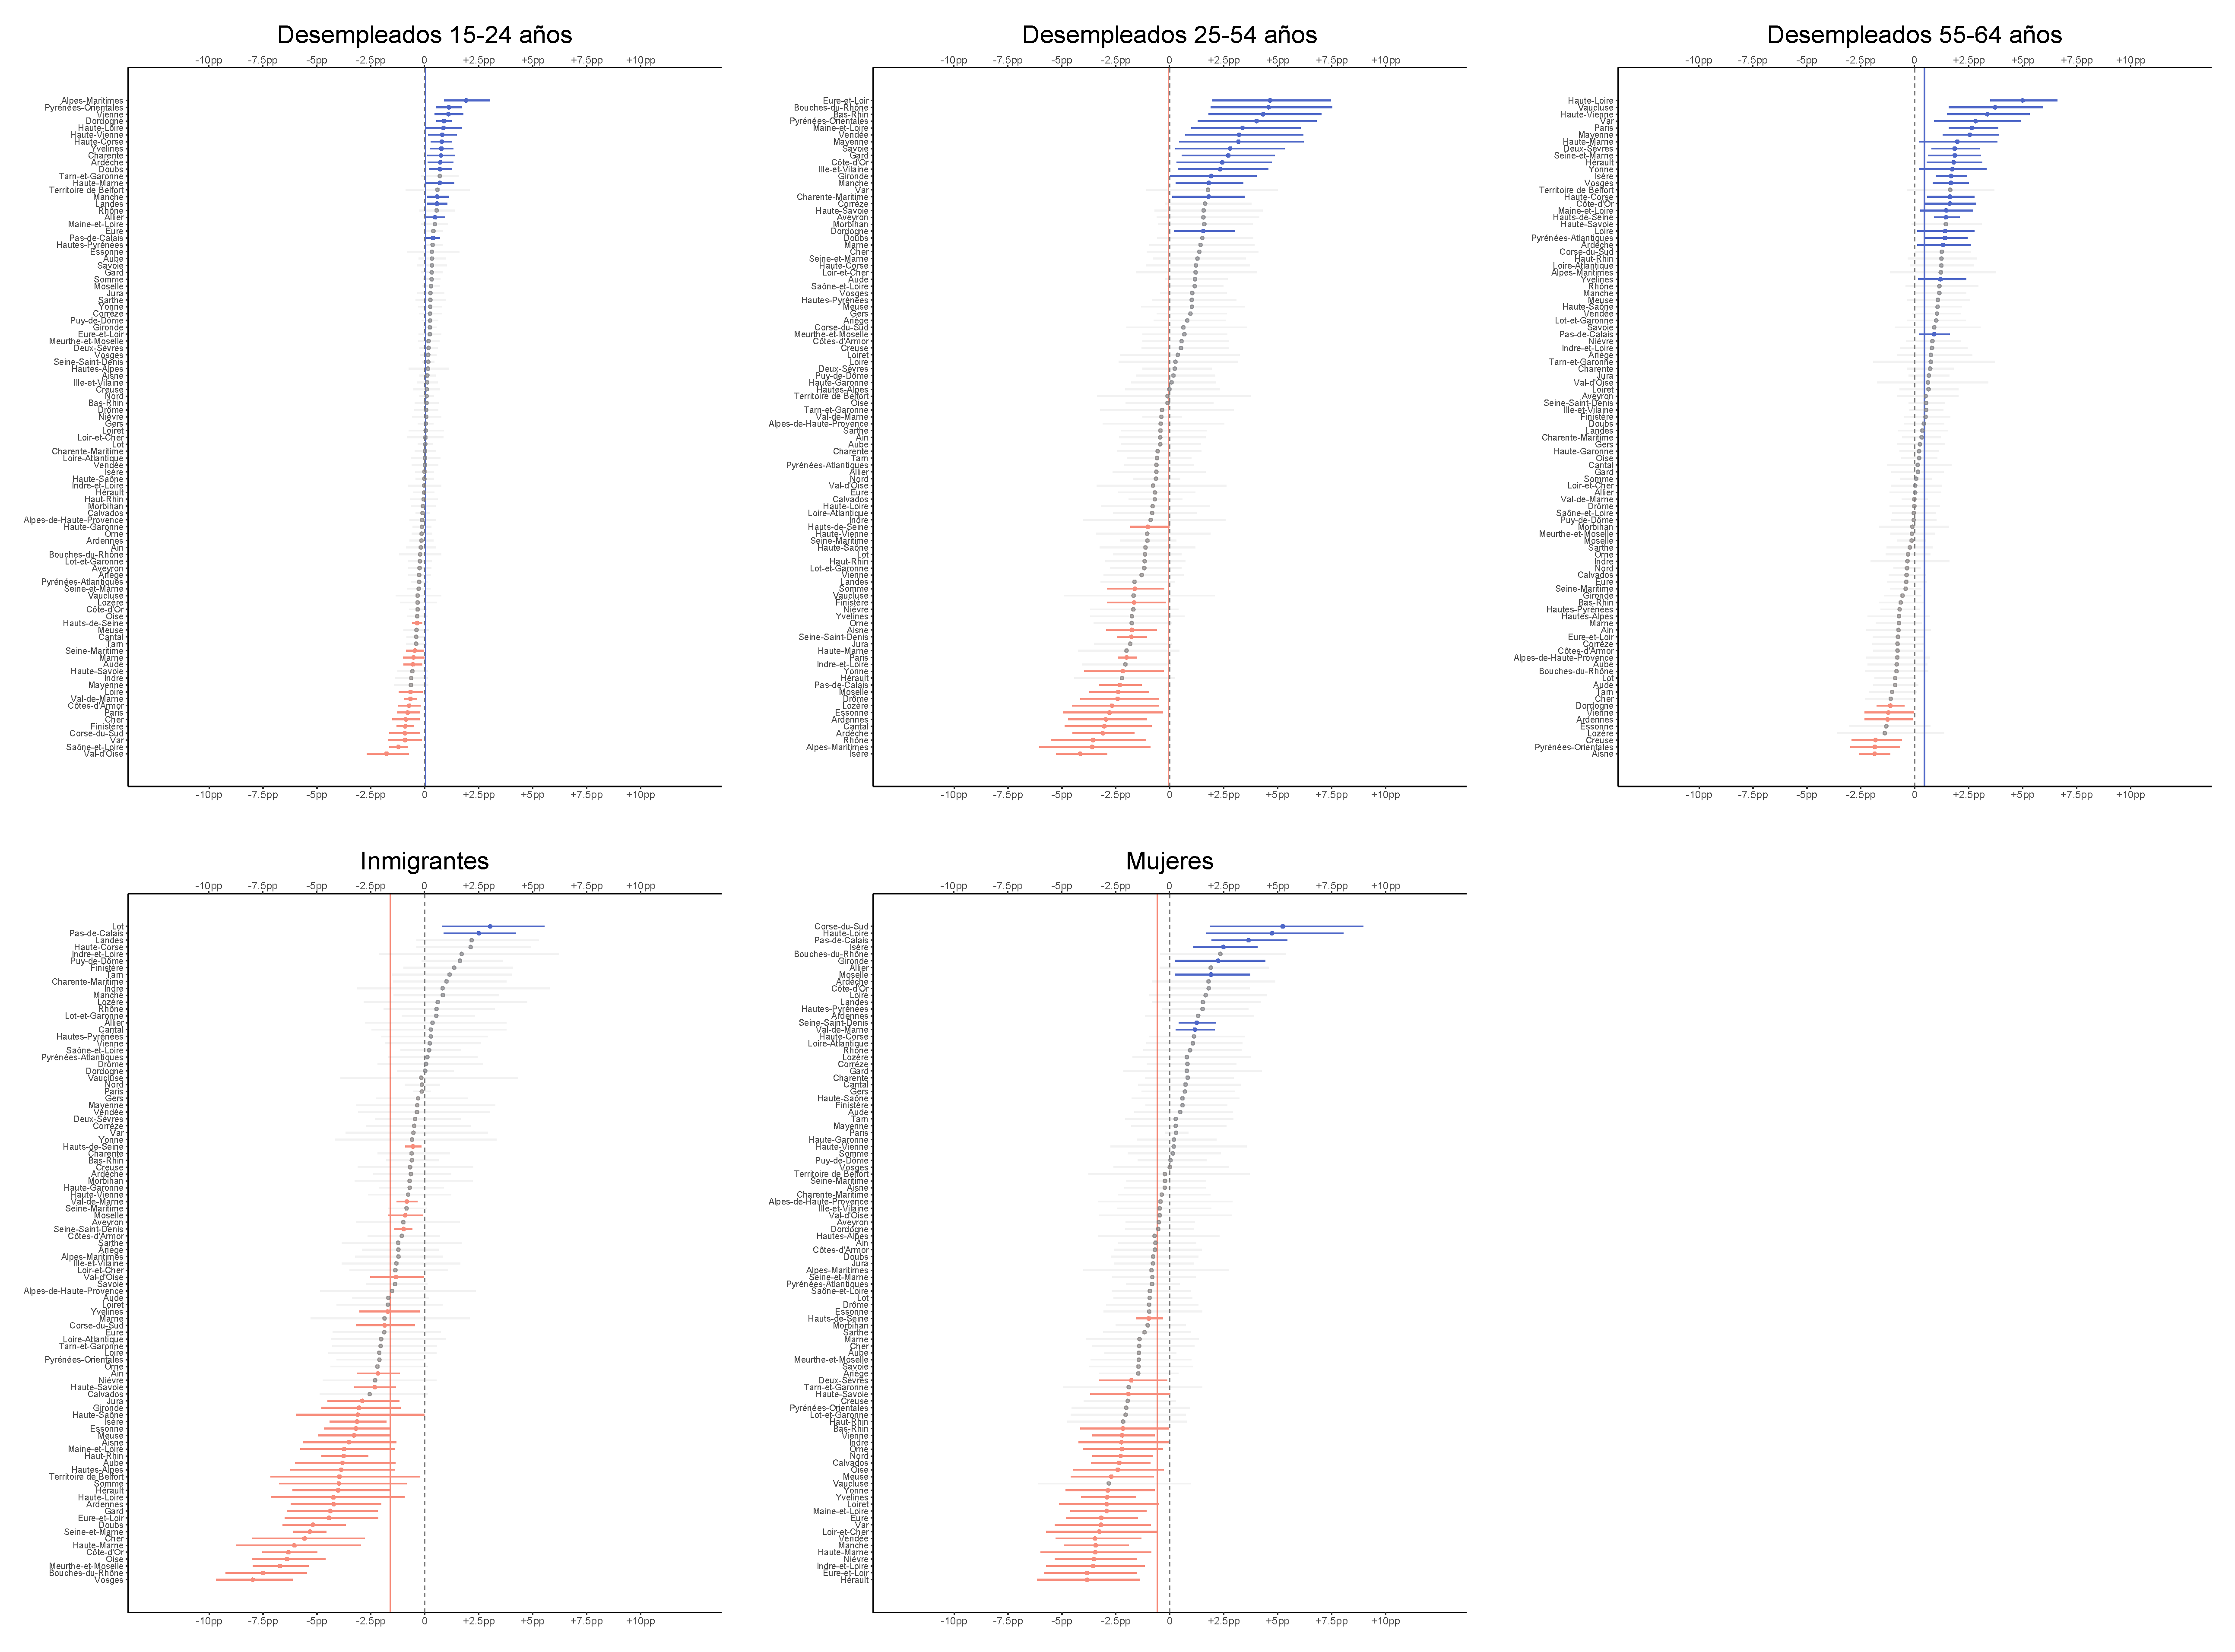
\includegraphics[width = 0.9\textwidth]{Figs/Efectos/Efectos_Dicotom_Modelo_H}
	\caption{Intervalos centrales de probabilidad al 95\%, 80\% y 50\% para los efectos de categorías dicotómicas por departamento francés bajo el modelo H. Los departamentos se ordenan para cada categoría por magnitud del estimador puntual que es el efecto mediano. Las distribuciones de colores rosa o azul representan que el efecto es significativo al 95\%. Las lineas verticales representan el efecto promedio a través de los departamentos. Fuente: elaboración propia.}
	\label{fig:Efectos_Dicotom}
\end{sidewaysfigure}

En el caso de la inmigración, las teorías del conflicto no parecen encontrar eco al observar los dorlings de la \textbf{Figura \ref{fig:Dorling_Efectos_Dicotom}}. Ciertamente aquí podríamos arriesgarnos a hablar de inferencia a nivel individual. Si una mayor proporción de inmigrantes adquieren derecho al voto, uno esperaría que no eligieran al partido NAP que resulta ser el FN. Por lo mismo, una mayor presencia de inmigrantes reduciría el voto frontista. Pero también existen las hipótesis que mencionan que el contacto con el inmigrante disminuye la xenofobia al comprobar que el otro no es tan diferente como se temía. En este sentido las explicaciones de un efecto indirecto de la presencia de inmigrantes parecerían más prometedoras que aquellas de xenofobia directa. Finalmente, para el caso de los desempleos observamos un claro contraste en la intensidad de los departamentos significativos entre el desempleo juvenil y el resto de categorías.\\ 

\begin{sidewaysfigure}
	\centering
	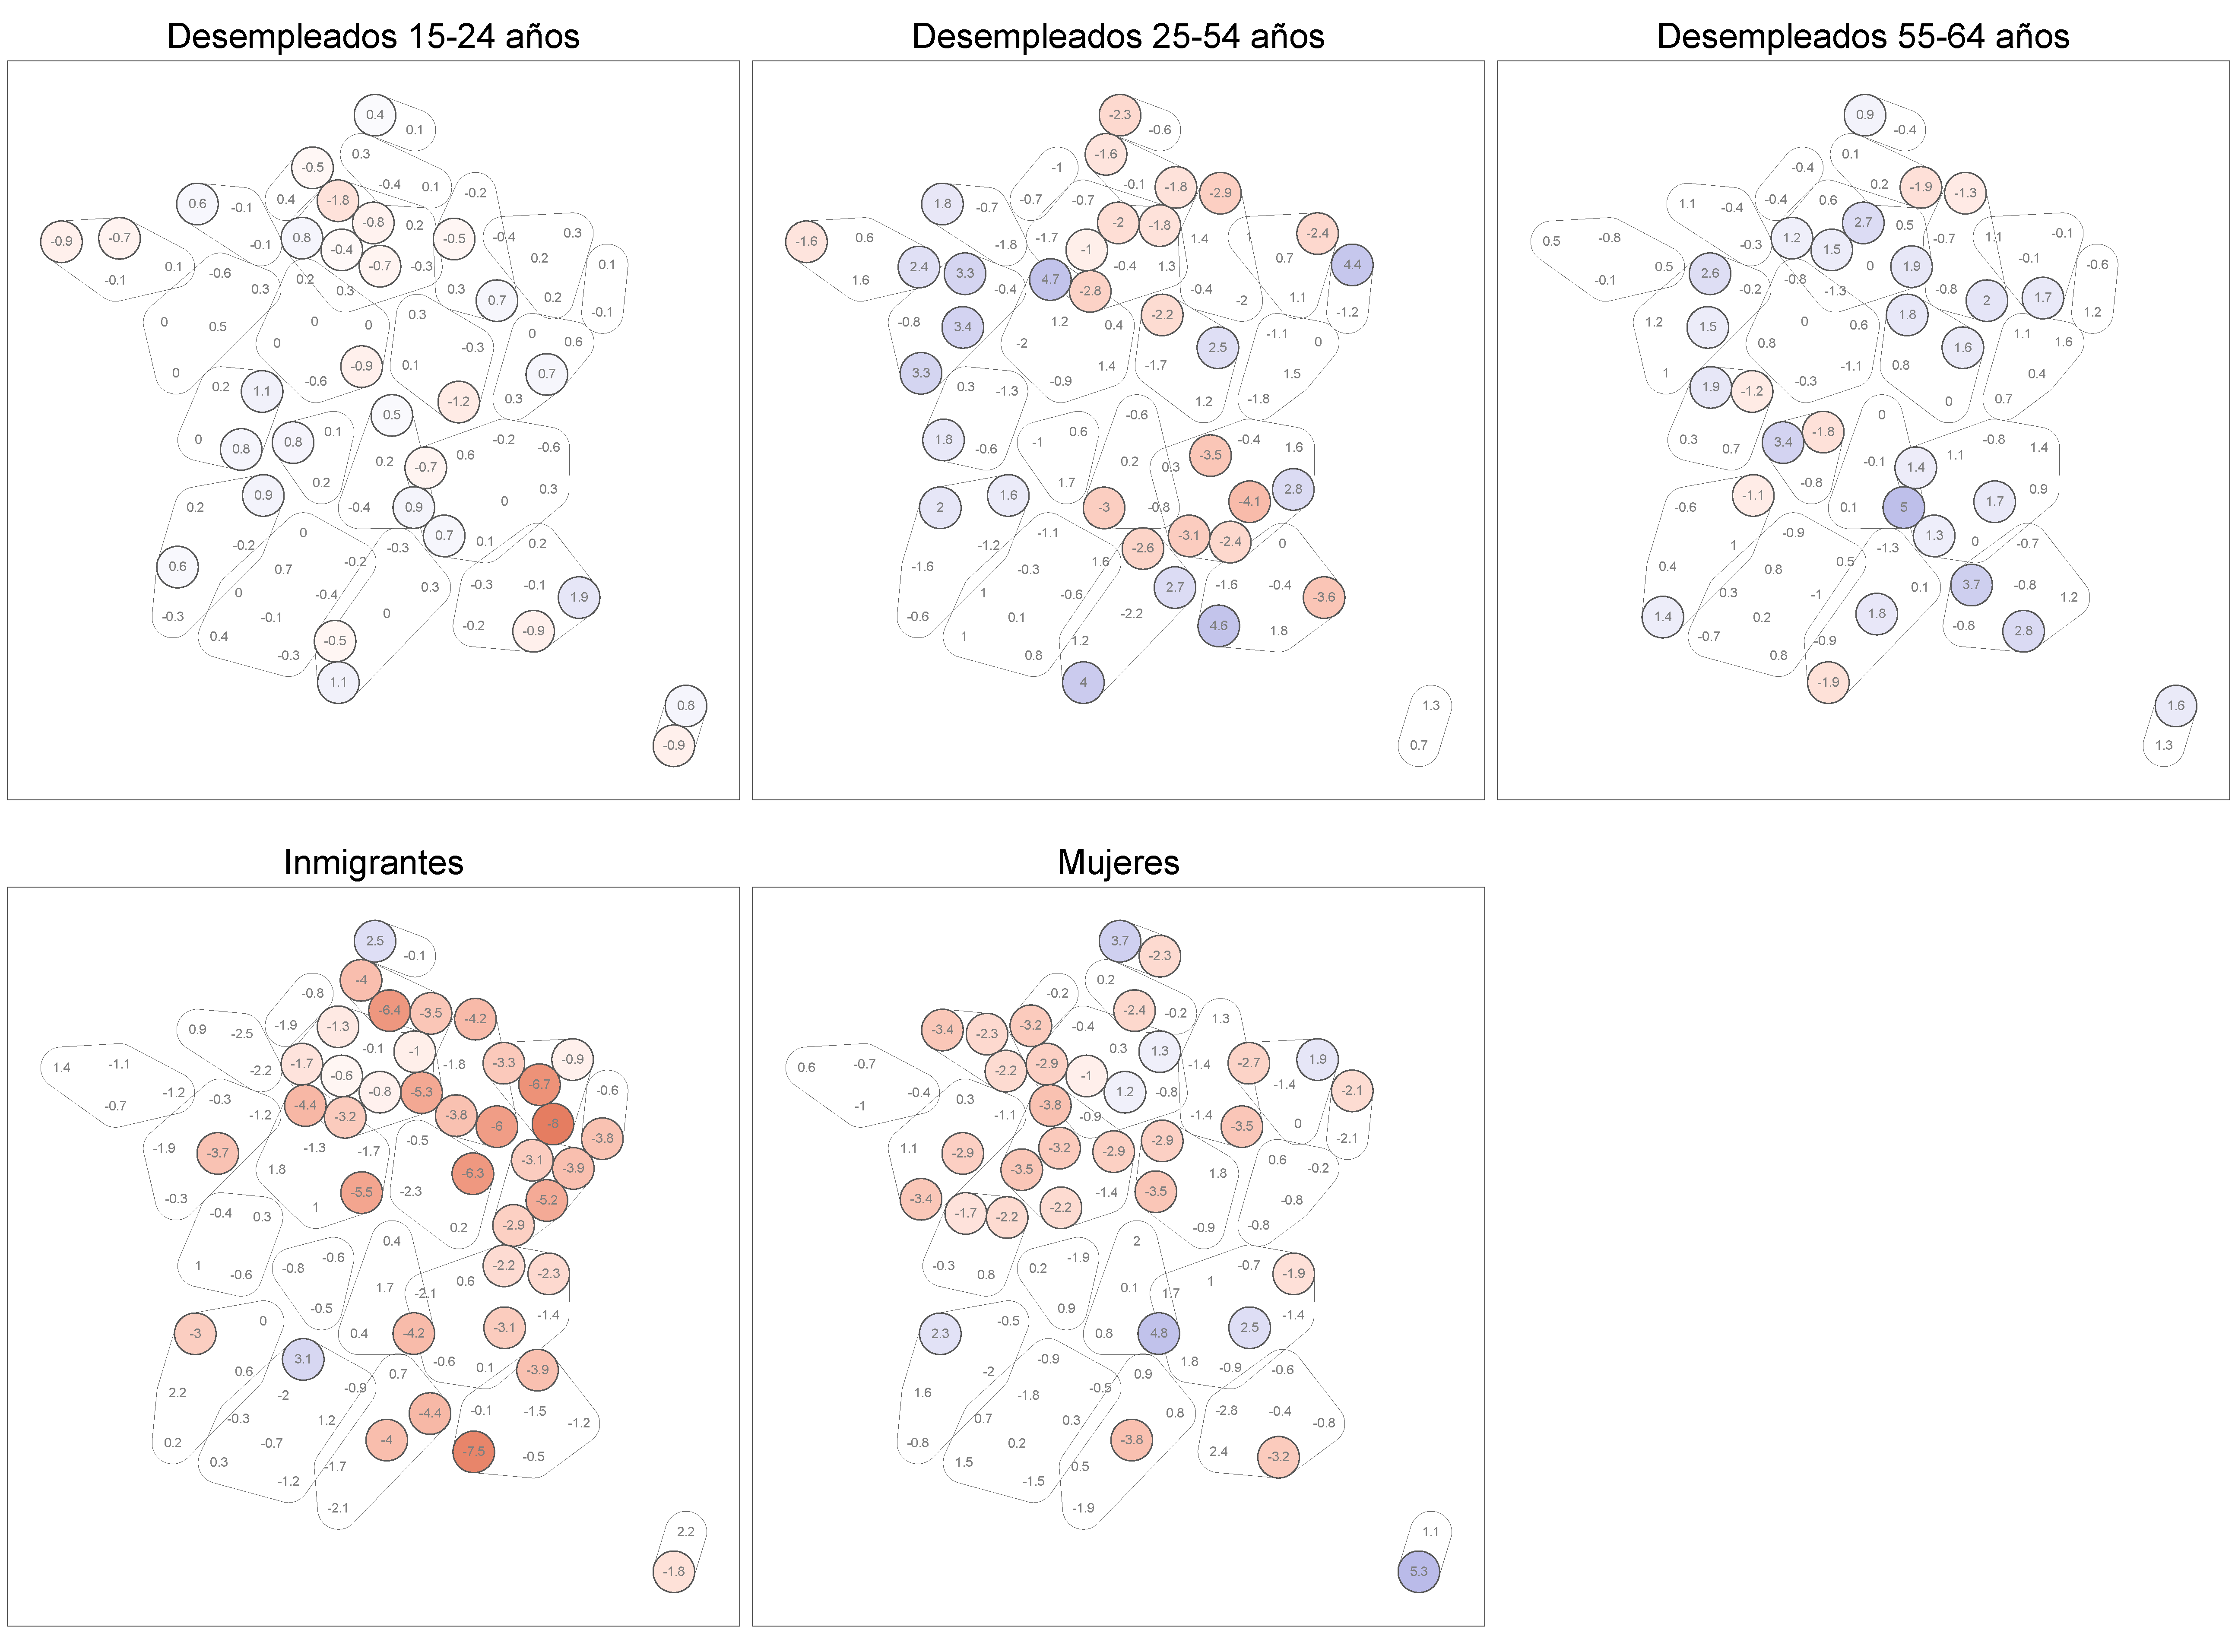
\includegraphics[width = 0.9\textwidth]{Figs/Efectos/Dorling_Efectos_Dicotom_Modelo_H}
	\caption{Estimaciones puntuales de los efectos de categorías dicotómicas por departamento francés bajo el modelo H, solo se colorean los efectos significativos. Fuente: elaboración propia.}
	\label{fig:Dorling_Efectos_Dicotom}
\end{sidewaysfigure}

Con base en este análisis gráfico procederé en el siguiente capítulo a resumir las conclusiones del estudio así como algunas reflexiones sobre trabajo futuro y extensiones. 